\newif\ifdebug
\debugfalse
%% (Master) Thesis template
% Template version used: v1.4
%
% Largely adapted from Adrian Nievergelt's template for the ADPS
% (lecture notes) project.


%% We use the memoir class because it offers a many easy to use features.
\documentclass[11pt,a4paper,titlepage]{memoir}

%% Packages
%% ========

%% LaTeX Font encoding -- DO NOT CHANGE
\usepackage[OT1]{fontenc}

%% Babel provides support for languages.  'english' uses British
%% English hyphenation and text snippets like "Figure" and
%% "Theorem". Use the option 'ngerman' if your document is in German.
%% Use 'american' for American English.  Note that if you change this,
%% the next LaTeX run may show spurious errors.  Simply run it again.
%% If they persist, remove the .aux file and try again.
\usepackage[american]{babel}

%% Input encoding 'utf8'. In some cases you might need 'utf8x' for
%% extra symbols. Not all editors, especially on Windows, are UTF-8
%% capable, so you may want to use 'latin1' instead.
\usepackage[utf8]{inputenc}

%% This changes default fonts for both text and math mode to use Herman Zapfs
%% excellent Palatino font.  Do not change this.
\usepackage[sc]{mathpazo}

%% The AMS-LaTeX extensions for mathematical typesetting.  Do not
%% remove.
\usepackage{amsmath,amssymb,amsfonts,mathrsfs}

%% NTheorem is a reimplementation of the AMS Theorem package. This
%% will allow us to typeset theorems like examples, proofs and
%% similar.  Do not remove.
%% NOTE: Must be loaded AFTER amsmath, or the \qed placement will
%% break
\usepackage[amsmath,thmmarks]{ntheorem}

%% LaTeX' own graphics handling
\usepackage{graphicx}

%% We unfortunately need this for the Rules chapter.  Remove it
%% afterwards; or at least NEVER use its underlining features.
%\usepackage{soul}

%% This allows you to add .pdf files. It is used to add the
%% declaration of originality.
\usepackage[final]{pdfpages}

%% Some more packages that you may want to use.  Have a look at the
%% file, and consult the package docs for each.
\input{extrapackages}

%% Our layout configuration.  DO NOT CHANGE.
\input{layoutsetup}

%% Theorem environments.  You will have to adapt this for a German
%% thesis.
\input{theoremsetup}

%% Helpful macros.
\input{macrosetup}

%% Make document internal hyperlinks wherever possible. (TOC, references)
%% This MUST be loaded after varioref, which is loaded in 'extrapackages'
%% above.  We just load it last to be safe.
\usepackage[linkcolor=black,colorlinks=true,citecolor=black,filecolor=black]{hyperref}

%%%%%% TODO

% Own packages
\usepackage[version=3]{mhchem}
\usepackage{mathtools}
\usepackage[]{algorithm2e}
\usepackage{framed}
\usepackage[]{units}
\usepackage{mdframed}
%\usepackage{subcaption}
\usepackage{epigraph}
%\usepackage{caption}

% TODO
% `` open, '' close, dots outside
%Range --
%\emph


%% Document information
%% ====================

\title{Parallelized Stochastic Reaction-Diffusion Simulations on GPGPU and multi-core CPU}
\author{\textbf{Fabian Güra}\\Munich School of Engineering\\Technische Universität München}
\thesistype{Bachelor's Thesis}
\advisors{Advisors ETH: Prof.\ Dr.\ Petros Koumoutsakos\\Jana Lipkov\'a, M.Sc.\ \\ Advisor TUM: Prof.\ Dr.\ Hans-Joachim Bungartz}
%\department{Computational Science and Engineering Laboratory}
\date{somewhen, 2014}

\begin{document}

\frontmatter

%% Title page is autogenerated from document information above.  DO
%% NOT CHANGE.
\begin{titlingpage}
  \calccentering{\unitlength}
  \begin{adjustwidth*}{\unitlength-24pt}{-\unitlength-24pt}
    \maketitle
  \end{adjustwidth*}
\end{titlingpage}

%% The abstract of your thesis.  Edit the file as needed.
\begin{abstract}
In this thesis the deterministic as well as the stochastic approach towards simulating chemical reaction-diffusion systems are presented. Apart from the underlying formalistic concepts two different implementations of the tau-leaping stochastic simulation algorithm are discussed. In addition to theoretical deliberation and accuracy validation, the performance of the algorithm in two parallel computing environments, namely Nvidia CUDA GPGPUs and OpenMP-enabled multi-core CPUs, is assessed. Throughout the complete thesis the Gray-Scott model is used as an example to illustrate various results. This reaction-diffusion system is not only subject to pattern-formation, but it is also of great interest due to is computational complexity and practical relevance. 
\end{abstract}

%% TOC with the proper setup, do not change.
\cleartorecto
\tableofcontents
\mainmatter

%% Your real content!
% Some commands used in this file
\newcommand{\package}{\emph}
\chapter{Introduction}
\label{ch:intro}
\chapterprecishere{"I had no idea this was going to be an accurate prediction, but amazingly enough instead of 10 [years] doubling, we got nine over the 10 years, but still followed pretty well along the curve."}{\hfill -- Gordon E. Moore\footnote{Computer History Museum Presents The 40th Anniversary of Moore's Law with Gordon Moore and Carver Mead (\url{http://goo.gl/4WT2ux})}

In 1965 Godon E. Moore, one of the founders of Intel, published his observation that the number of transistors on a chip of same size doubles approximately every 24 months and predicted similar exponential growth for the future \cite{moore_cramming_1965}. The so-called ``Moore's Law'' is illustrated in figure \ref{fig:moore_data}. A higher level of integration usually goes hand in hand with increasing performance. The availability of greater computational capabilities does not only accelerate existing solutions, but may enable applications from a variety of research fields that were previously impossible to realize or had been completely out of scope a few years ago. 

One of these fields is biochemistry. Over the years, computational methods have become a valuable and integrative tool that is by no means able to completely replace traditional laboratory experiments, but can help to gain deeper insight into complex reaction mechanisms that can hardly be understood from experiments alone, but dominate the comportment of the system of interest. Nowadays, apart from reproduction and model validation, it is possible to derive predictions for the behaviour of a system subject to parameters that have not yet been studied in experiments. The approach does not only help to cut costs, but can greatly increase flexibility and pace of research in this field.  

\begin{figure}
\centering
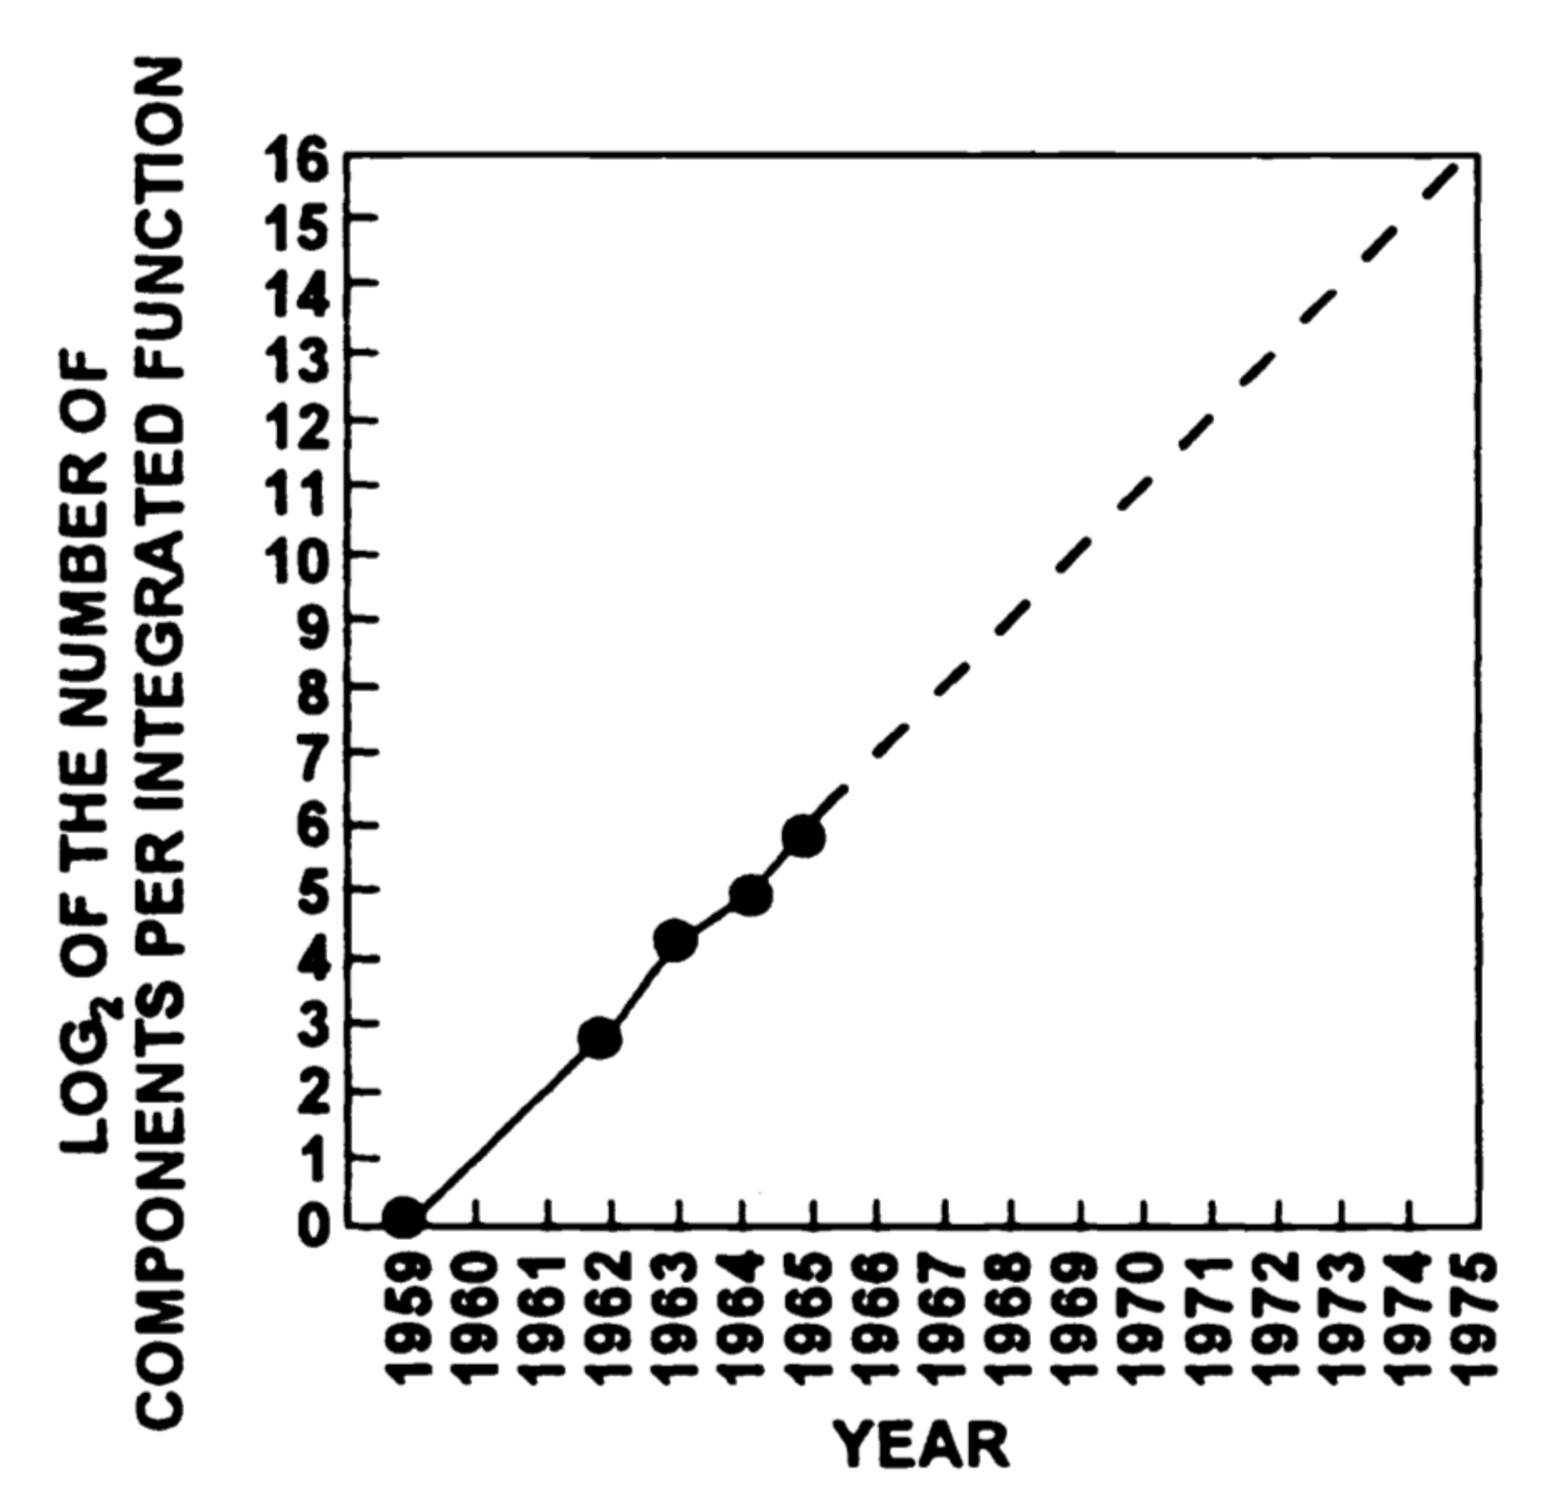
\includegraphics[width=0.7\textwidth]{images/original_moore.eps}
\caption{Original illustration of ``Moor's Law''. Figure taken from \cite{moore_cramming_1965}.}
\label{fig:moore_original}
\end{figure}

\begin{figure}
\centering
% l b r t
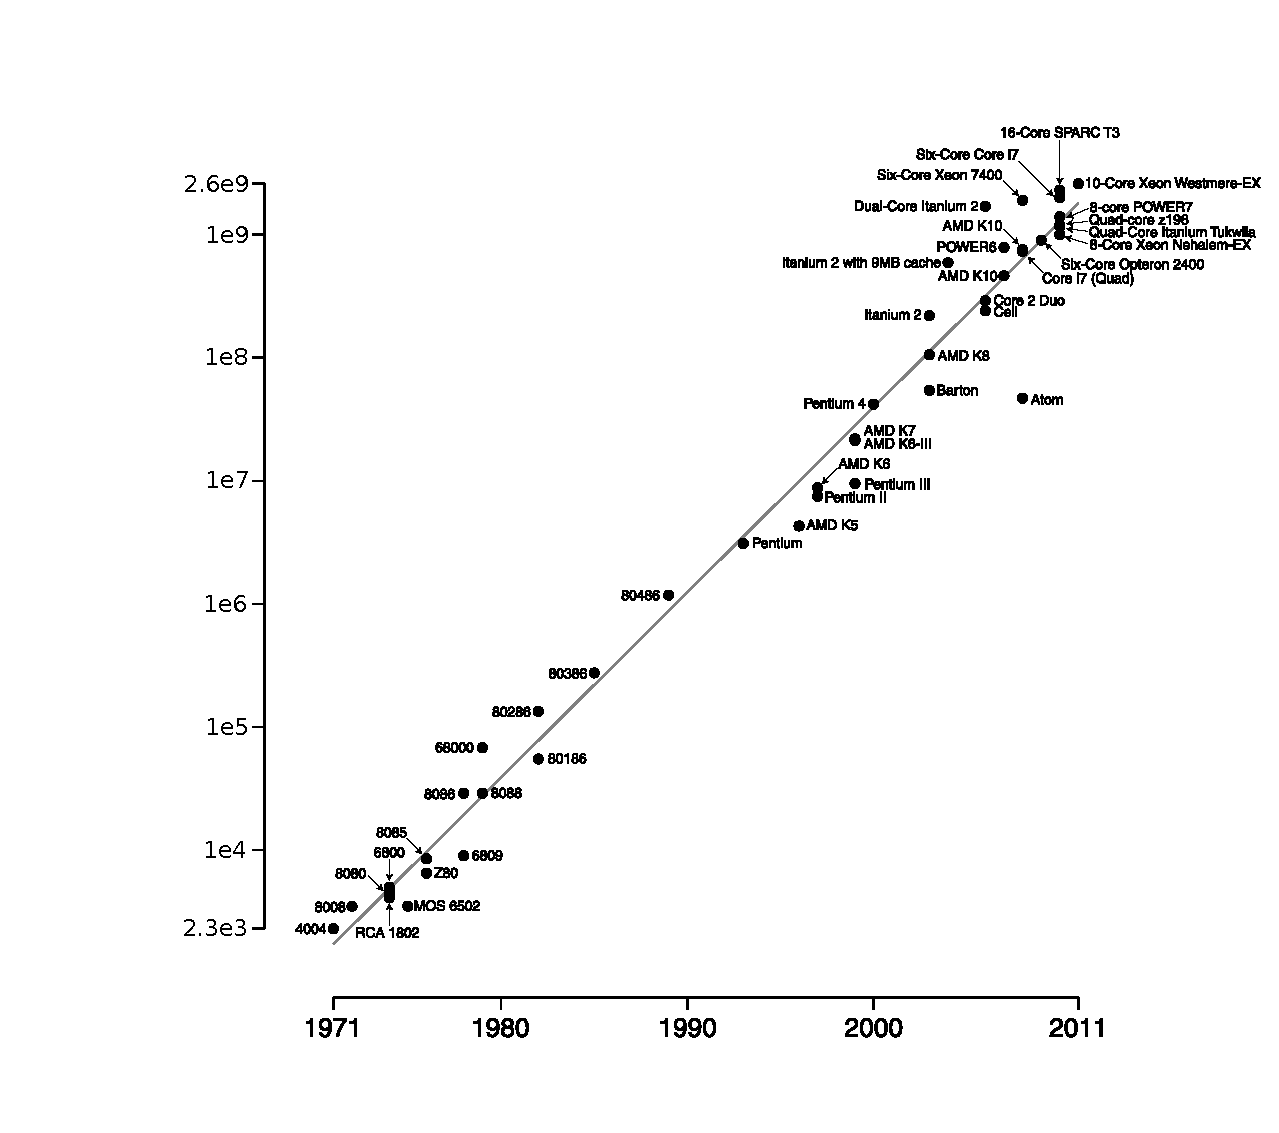
\includegraphics[trim = 20mm 10mm 0mm 0mm, clip,width=0.95\textwidth]{images/TransistorCount.eps}
\caption{Transistor counts of selected microprocessors introduced in the years 1971-2011. The diagonal line represents Moore's law. Figure taken from \cite{wgsimon_transistor_2011} (modified).}
\label{fig:moore_data}
\end{figure}

In the emerging field of computational biochemistry two fundamentally different approaches are used to derive the dynamic evolution of a system over time from a mathematical model: deterministic and stochastic simulation. The former, often considered the `classical' way, is based on a macroscopic description of the reactive species. The system is represented by a set of differential equations which can be solved numerically to gain insight into its dynamic behaviour. The latter, a more recently proposed and popularized approach, is based on the intrinsic randomness chemical species are subject to on a microscopic level. In the context of probability theory and statistics, the next reaction to fire as well as the according point in time can be modeled by means of correctly-distributed random variables. 

Over the course of centuries numerous fundamental theoretical results and efficient numerical methods for solving differential equations have been presented. Today, in consequence, systems of reasonable size can be solved accurately on affordable computing hardware in a relatively short amount of time. On the other hand, deterministic methods are considerably more expensive from a computational point of view. Furthermore, for system configurations where macroscopic concepts such as concentration are a valid approximation to the microscopic system dynamics, the averaged results of stochastic simulations often converge to the deterministic solution. One may therefore be tempted to question the relevance of the stochastic approach in practice. However, in cases where system dynamics is dominated by the particles of one or more species available only in small quantities, deterministic models cannot be used. In fact stochastic algorithms are needed to correctly simulate the temporal evolution of most biological systems. Stochastic effects arising from small molecular concentrations can only be considered by a non-deterministic approach. Examples of successful applications include genetics \cite{mcadams_stochastic_1997}, cellular signal transduction \cite{erban_signal_2005} and drug delivery \cite{ford_multi-scale_2011}. 

In practice a great variety of these processes can be modeled in terms of reaction and diffusion. Particles close to one another can collide and react according to prescribed reaction channels. Diffusion, on the other hand, macroscopically describes the spatial movement of molecules in the direction of the negative concentration gradient due to microscopic effects such as Brownian motion. The methods presented in the framework of this thesis are applicable for generic reaction-diffusion systems. To maintain a reasonable scope, however, a special focus is placed on the Gray-Scott model \cite{gray_autocatalytic_1984, pearson_complex_1993}. This primary example is of great interest due to its ability to exhibit pattern formation caused by an embedded activator-inhibitor process. Pattern formation as a form of self-organization ``can be considered the complement of the second law of thermodynamics\footnote{"The entropy of a closed system never decreases"} explaining the emergence of order from disorder instead of disorder from order'' \cite{mainzer_local_2013}. In practice this mechanism was observed in follicle spacing on mice skin \cite{sick_wnt_2006}. It can be used to describe pigmentation pattering in mammals \cite{murray_mathematical_2002}. Reaction-diffusion models have recently been used to simulate signalling pathways in eukaryotic cells \cite{takahashi_spatio-temporal_2010}. 

For his original prediction Moore considered a time span of ten years into the future (see figure \ref{fig:moore_original}). As of today (July 2014), Moor's Law is still considered to be valid \cite{techradar_moores_2014}. However, it is a common misunderstanding that computing power of microprocessors doubles at the same rate. Not the level of integration is the main driver of performance, but the processor's clock speed is. The latter has an enormous influence on the system's energy efficiency and since it is bound by the amount of heat a CPU cooler can dissipate, (starting in around 2005/06) a novel approach was introduced to the mainstream market: multi-core CPUs. This paradigm shift requires developers to explicitly write code that can make use of multiple parallel execution units. Another more recent trend in scientific computation is General-purpose Computing on Graphics Processing Units (GPGPU). Considering raw computational power (i.e.\ the number of floating point operations per second, FLOP/s) GPUs easily outperform CPUs. 

Due to the great computational complexity of stochastic simulation algorithms parallel platforms must be considered in order to simulate systems whose enormous complexity was previously considered prohibitive. In this thesis a simulator is presented that can make use of both, multi-core CPU and GPU, to accelerate stochastic reaction-diffusion simulations. The implementation depends on the OpenMP standard and Nvidia CUDA, respectively. Even though optimization techniques were used and the results of performance analysis is given, this work will not answer the question of which platform is suited better for stochastic simulations. The presented application is far from being perfect on both platforms. The goal of the project is merely to give an overview about available techniques and demonstrate results that can be achieved in a time-limited academic project. 

The structure of this thesis is as follows: In chapter 1, a compact overview about the topics and the scope of this thesis was given. In chapter 2, theoretical aspects of both approaches are derived and important results are cited. It is therefore the foundation for the two following chapters: In chapter 3, the implementation details and ideas incorporated into the developed programmes as well as the platforms they are targeted at are presented. In the subsequent chapter the tools are validated by comparison to analytic solutions of model examples. In addition, the more complex Gray-Scott model is simulated to assess performance on the different platforms and to demonstrate the pattern formation mechanism. The final chapter briefly summarizes the results of the thesis and gives an outlook on possibilities, trends and ideas to further improve the presented methods.
\chapter{Approaches to Simulating Chemical Reaction-Duffusion Systems}
\chapterprecishere{"Theory without practice cannont survive and dies as quickly as it lives. He who loves practice without theory is like the sailor who boards ship without a rudder and compass and never knows where he may cast."}{\hfill -- Leonardo da Vinci \cite{brym_sociology:_2006}}

In this chapter, the two fundamental approaches towards modeling chemical reaction-diffusion systems are presented. On the one hand, deterministic models based on rate laws and differential equations are the traditional way of describing the dynamic evolution of a system over time. Stochastic models, on the other hand, are based on the intrinsically random behavior of such systems. Unlike in the deterministic case, running a stochastic simulation algorithm twice gives two possible, but usually completely different solutions, each representing one possible scenario of how the system may develop over time in reality. Often averaging the states obtained by a great number of stochastic simulations yields the solution of the deterministic simulation, however, this is not always the case. For some models, especially those representing biochemical systems, stochastic simulations can give more insight. Whenever the presence of one or more species can heavily affect the dynamic evolution of the overall system (i.e.\ by enabling or disabling a specific reaction channel), but the absolute number of molecules is low, the intrinsic randomness in particle movement has to be considered. Stochastic effects can only be modeled by a stochastic approach, deterministic algorithms are not applicable in this case. 
%
%\section{Illustrative Model: The Gray-Scott System}
\section{Illustrative Model: The Gray-Scott System}
Throughout this thesis, the Gray-Scott reaction system described in \cite{pearson_complex_1993} will be used as a primary example to illustrate the presented techniques, algorithms and results. 

The chemical reaction system consists of two species U and V subject to the reactions as described in the following: \\
\begin{align}
\label{eq:r1}
\cee{\emptyset{} &->[F] U} \\
\label{eq:r2}
\cee{U &->[F] \emptyset} \\
\label{eq:r3}
\cee{V &->[F+\kappa] \emptyset} \\
\label{eq:r4}
\cee{U + 2V &->[\rho] 3V}
\end{align}
with positive reaction rate constants $F$, $\kappa$ and $\rho$.

The two species U and V are also subject to diffusion. Approaches towards modelling this spatial dependency of the system will be discussed in chapters (ref) and (ref) for the deterministic and the stochastic case. 

The reactions given above can be interpreted as follows: Reactions \eqref{eq:r1} and \eqref{eq:r2} describe degradation and production of U particles, respectively. Since they are the opposite to each other, the process of production and degradation of U is reversible. Equation \eqref{eq:r3} describes degradation of V particles. Note that there is no direct production of V in the system. Finally, reaction \eqref{eq:r4} describes the autocatalytic\footnote{A reaction is said to be autocatalytic if it is catalyzed by its products \cite[pg.\ 907]{atkins_physical_2009}. In this example, V particles can only be generated if there are already some available in the system to catalyze the reaction.} conversion of U particles to V particles. The symbol $\emptyset$ represents species that are available in excess (i.e.\ not rate-limiting), but are of no further interest for the modeled process. 

The Gray-Scott model is of great interest since it
\begin{itemize}
\item can be used to describe real-world phenomena.
\item is subject to pattern formation (for certain parametrizations).
\item is computationally expensive due to spatial dependencies.
\end{itemize}
All these properties will be examined more closely throughout the thesis. 
%
%
%
%
%
%
%
%
\ifdebug

Reasoning: Molecules must collide before they can react (for 2nd and higher order). $\rightarrow$ reaction within compartment makes sure that molecules are close to each other (have a chance to collide)

\underline{Reactions}
\begin{align}
\label{eq:r1}
\cee{\emptyset{} &->[F] U_{i,j,k}} \\
\label{eq:r2}
\cee{U_{i,j,k} &->[F] \emptyset} \\
\label{eq:r3}
\cee{V_{i,j,k} &->[F+\kappa] \emptyset} \\
\label{eq:r4}
\cee{U_{i,j,k} + 2V_{i,j,k} &->[\rho] 3V_{i,j,k}}
\end{align}
with positive reaction rate constants $F$, $\kappa$ and $\rho$.

\underline{Diffusion}
\begin{align}
\label{eq:d1}
\cee{S_{i,j,k} &<->[d_S] S_{i\pm{}1,j,k}} \\
\cee{S_{i,j,k} &<->[d_S] S_{i,j\pm{}1,k}} \\
\cee{S_{i,j,k} &<->[d_S] S_{i,j,k\pm{}1}}
\label{eq:d3}
\end{align}
for the two species $\text{S} \in \{\text{U, V}\}$ with positive diffusion constants $d_\text{U}$ and $d_\text{V}$. 

The spatial dependency of the system is reflected by the compartment index (i,j,k). In a uniform, three-dimensional grid with spacing $h$, compartment $C_{i,j,k}$ is equal to the cube $\left[(i-1)h,ih\right] \times \left[(j-1)h,jh\right] \times \left[(k-1)h,kh\right]$. It is assumed that only particles close to each other (i.e.\ within a compartment) can  react according to equations \eqref{eq:r1} - \eqref{eq:r4}. Equations \eqref{eq:d1} - \eqref{eq:d3}, on the other hand, describe how particles can migrate from one compartment to another. Diffusion is therefore modeled as a jump process between neighboring compartments. Compartment-based simulation of diffusion as well as its relation to Fick's law of diffusion will be introduced in more detail in chapter \eqref{stochdiff}. 
\fi
%\section{Deterministic Simulation}
\section{Deterministic Simulation}
\label{ch:determ_sim}
The traditional way of simulating chemical models is to solve a system of differential equations. The solution obtained is deterministic in the sense that it is, for given parameters, unique and accurately reproducible (up to possible numerical errors). 
\subsection{Reaction Rate Equations}
Let there be a system with species $X_i$, $i=1, \ldots,N$ and reactions $R_j$, $j=1, \ldots,M$. The state of the system $\vec{x}(t)$ at time $t$ is determined by the concentrations\footnote{Unlike in chemical literature where concentration is usually defined as "number of moles/volume", in this thesis a more general concept of concentration scaling is introduced (see chapter \ref{ch:scaling}).} of its species $X_i$. Let $x_i = [X_i]$ denote the concentration of species $X_i$. For the moment, the system is considered to be well-stirred, i.e.\ the system is spatially homogeneous with respect to the concentrations of all species. A spatial effect in inhomogeneous systems, namely diffusion, will be considered in chapter \ref{det_diff}. 

By applying the \textit{Law of mass action}, one can find $N$ differential equations that describe the rate of change of concentration over time for every species $X_i$:
\begin{equation}
\frac{dx_i}{dt} = \sum_{j=1}^M v_{ij}f_j(\vec{x})
\end{equation}
$v_{ij}$ denotes the number of particles of species $X_i$ that are created ($v_{ij} > 0$) or consumed ($v_{ij} < 0$) in reaction $R_j$. $f_j$ is the reaction rate of $R_j$ which in general depends on the current state of the system. 

For simple ("elementary") reactions, the reaction rate is proportional to the product of the concentrations of the reactant species raised to the power of the respective stoichiometric coefficients. Considering for example the reaction $\ce{ 2A -> B}$, one has $\frac{da}{dt} = -2 k a^2$ and $\frac{db}{dt} = k a^2$. 

Applying this formalism to the reactions \eqref{eq:r1} - \eqref{eq:r4} from the Gray-Scott model, the system can be represented by the following differential equations:
\begin{align}
\label{eq:ode1}
\frac{du}{dt} &= - \rho u v^2 + F(1-u) \\
\label{eq:ode2}
\frac{dv}{dt} &= \rho u v^2 - (F + \kappa) v
\end{align}
In order to uniquely determine the solution of the system, the mathematical model is completed by introducing initial conditions:
\begin{equation}
\vec{x}(t = 0) = \vec{x}_0 = \begin{bmatrix}u_0 & v_0\end{bmatrix}^T
%\vec{x}(t = 0) = \vec{x}_0 = \lbrack u_0 \: v_0 \rbrack^T
\end{equation}

\subsection{Steady State Analysis}
Steady state analysis is a practical way to gain an initial insight into how a chemical system may develop in time. In order to better understand the primary example of this thesis, the Gray-Scott model shall now be analyzed with this technique. 

A steady state $\vec{x}_s$ of a system of ordinary differential equations (ODEs) of the form $\frac{d\vec{x}}{dt}=f(\vec{x},t)$ has to satisfy $f(\vec{x}_s,t)=\vec{0} \ \forall t \geq 0$. Considering the equations \eqref{eq:ode1} and \eqref{eq:ode2}, it is obvious that $\vec{x}_{s1} = \begin{bmatrix} 1.0 & 0.0\end{bmatrix}^T$ is a trivial steady state. When all molecules of species V are gone (or there have never been any), the autocatalyzed reaction \eqref{eq:r4} cannot fire any more and the concentration $v$ will remain at zero. The system is therefore reduced to the single ODE $\frac{du}{dt} = F (1-u)$, where the right hand side is 0 iff\footnote{"if and only if"} $u=1$. \\
Throughout the simulations which are carried out in chapter \ref{ch:4}, the parameter values proposed in \cite{rossinelli_accelerated_2008} ($F = 0.04$, $\kappa = 0.06$ and $\rho = 1.0$) will be used. For this setup, another steady state is located at $\vec{x}_{s2} = \begin{bmatrix}0.5 & 0.2\end{bmatrix}^T$. Detailed calculations can be found in the appendix (\ref{ch:app1}). 

To asses the stability of the steady states, the eigenvalues of the Jacobian evaluated at these points in phase space are needed. In the trivial case on obtains $\lambda_{11} = -0.1$ and $\lambda_{12} = -0.04$. Since the real part of both eigenvalues is less than zero (i.e.\ $\Re(\lambda_{1i})<0, i=1,2$), the steady state is stable. The eigenvalues of the non-trivial pole are $\lambda_{21} = 0$ and $\lambda_{22} = 0.02$, in consequence the steady state is unstable. 

Considering initial conditions $\vec{x}_0 = \begin{bmatrix}0.5 & 0.25\end{bmatrix}^T$ and the results of the calculations above one can predict that the system will move towards the steady state $\vec{x}_{s1}$ over time. This behaviour can be observed in figure \ref{fig:gs_time_evolution} after the transient response has gone away. Figure \ref{fig:phasespace} illustrates the corresponding trajectory in phase space. It can be concluded that diffusion is necessary for complex pattern formation in the Gray-Scott model. An advanced analysis of the involved mechanism (i.e.\ Turing bifurcation) can be found in \cite{vastano_turing_1988}. 

\begin{figure}
\centering
%l b r t
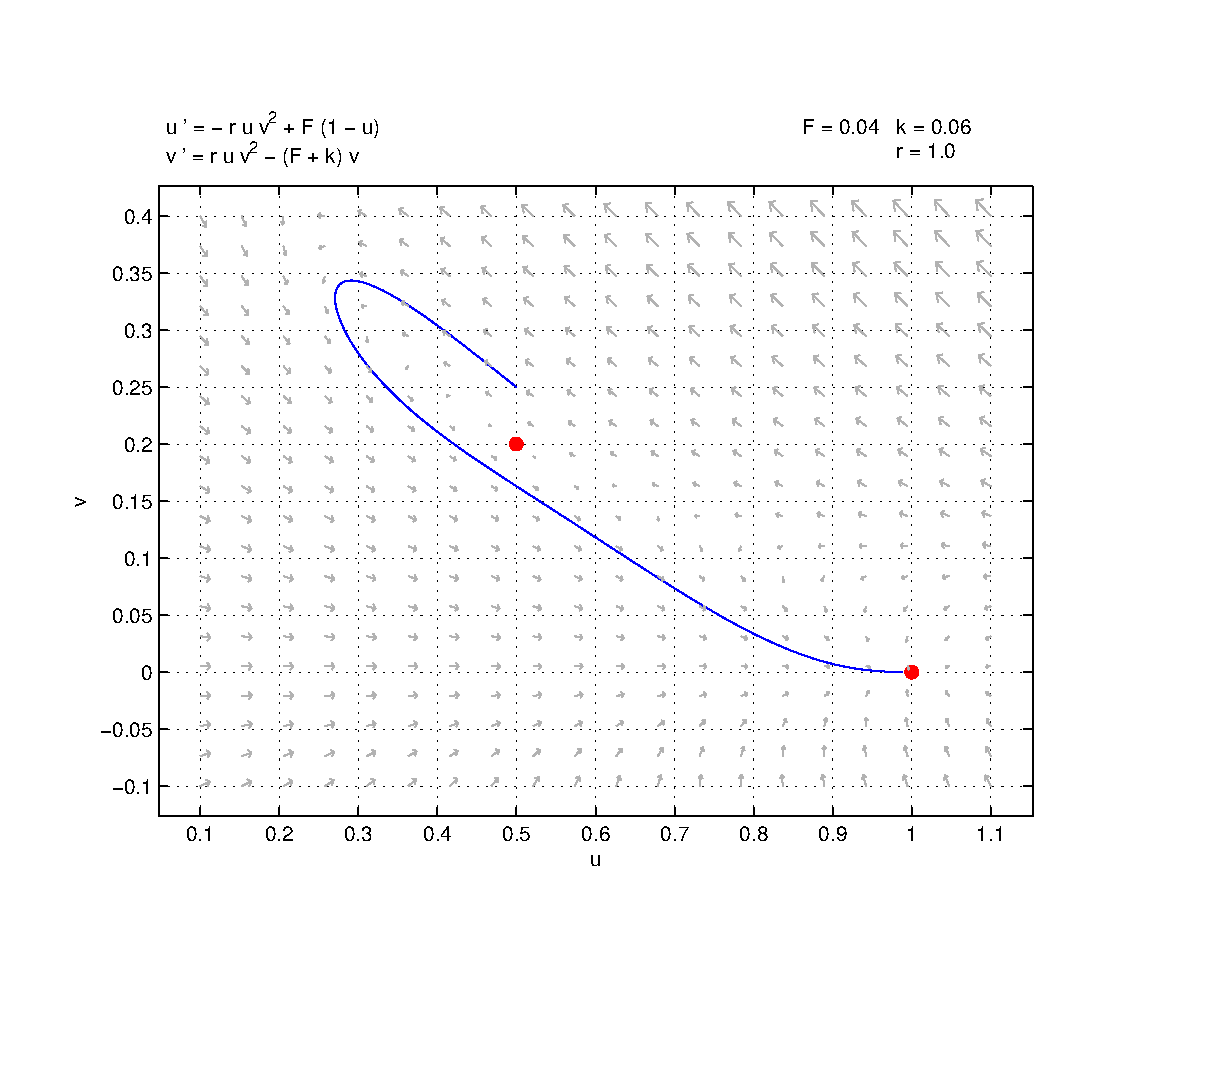
\includegraphics[trim = 5mm 25mm 20mm 5mm, clip, width=3cm,width=\textwidth]{images/phasespace.eps}
\caption{Phase space plot of the Gray-Scott local reaction system. Trajectory starts at $\vec{x}_0$. Red dots mark steady states. }
\label{fig:phasespace}
\end{figure}

%\subsection{Diffusion and Fick's Law}
\subsection{Diffusion and Fick's Law}
\label{det_diff}
The term diffusion describes the phenomenon that matter migrates in the direction of the negative concentration gradient. In consequence, inhomogeneities in the system tend to spread over time and gradients disappear (cite Atkins, pg.\ 770). Diffusion is an integral part of the Gray-Scott model since it is essential for the pattern formation mechanism. In the following, a deterministic description for diffusion (Fick's law) will be derived to incorporate the phenomenon into the reaction rate equations \eqref{eq:ode1} and \eqref{eq:ode2} given above. 

Let there be a cubic tube filled with a solution of some species A. The tube stretches along the $x$-Axis. The extent in the two other directions is negligibly small and so are possible concentration inhomogeneities in this plane. On the left end, the concentration $a = [A]$ is high, on the right end it is low. Figure \eqref{fig:fickslaw} illustrates the setup. Considering a slab of length $l$ ranging from $x_s$ to $x_s + l$ perpendicular to the $x$-Axis, the change of concentration inside the slab in some infinitesimal time interval is equal to the influx through the cross-sectional area $A$ at $x = x_s$ minus the flux out of the slab at $x = x_s + l$:
\begin{align}
\label{eq:diff_flux}
\frac{\partial a}{\partial t} = \frac{J(x_s) A dt}{A l dt} - \frac{J(x_s + l) A dt}{A l dt} = \frac{J - J'}{l}
\end{align}
The flux $J(x)$ at position $x$ is proportional to the negative concentration gradient $\frac{\partial a}{\partial x}$ at $x$. Using this relation gives 
\begin{align}
\begin{split}
J - J' &= -D \frac{\partial a}{\partial x} + D \frac{\partial a'}{\partial x} \\
&= -D \frac{\partial a}{\partial x} + D \frac{\partial}{\partial x} \left\{ a + \frac{\partial a}{\partial x} l \right\} 
= D l \frac{\partial^2 a}{\partial x^2}
\end{split}
\end{align}
with positive diffusion constant $D$. 

\begin{figure}
\centering
\includegraphics[width=\textwidth]{images/fickslaw.pdf}
\caption{Illustration of the setup used to derive Fick's law of diffusion}
\label{fig:fickslaw}
\end{figure}

By substituting this relation back into \eqref{eq:diff_flux} and by passing the limit $l \to 0$, one obtains the one-dimensional version of Fick's law of diffusion:
\begin{align}
\frac{\partial a}{\partial x} = D \frac{\partial^2 a}{\partial x^2}
\end{align}
In the generalized 3D case, the spatial derivative term turns into the Laplace operator $\Delta u = \frac{\partial^2 u}{\partial x^2} + \frac{\partial^2 u}{\partial y^2} + \frac{\partial^2 u}{\partial z^2}$: 
\begin{align}
\frac{\partial a}{\partial t} = D \Delta u
\end{align}

The complete Gray-Scott model is then discribed by the following partial differential equations:
\begin{gather}
\frac{\partial u}{\partial t} = D_u \Delta u - \rho u v^2 + F(1-u) \\
\frac{\partial v}{\partial t} = D_v \Delta v + \rho u v^2 - (F+\kappa) v
\end{gather}
where $D_u$ and $D_v$ are positive diffusion constants of the species U and V, respectively.
%\section{Stochastic Simulation}
\section{Stochastic Simulation}
\label{ch:stochsim}
Another, more recently proposed way of simulating chemical systems are stochastic simulation algorithms (SSA) \cite{gillespie_general_1976}. Unlike in the deterministic case, the solution obtained is not unique, but it only represents one possible way the system can develop in time. In theory, i.e.\ on a computer with infinite precision equipped with a perfect source of random numbers, the probability that a SSA will give exactly the same result in two or more independent runs is zero. In practice, however, a computer is a highly deterministic machine with finite precision. Therefore, the number of possible solutions of a SSA is finite. Since most computers don't have true random generators built in, pseudo-random number generators (PRNG) have to be used. PRNGs can create a sequence of numbers $Z_i$ that is random in the sense that it is compliant with a given probability distribution (usually $Z \sim \mathcal{U}(0,1)$) according to a variety of statistical tests (i.e.\ the TestU01 Big Crush testing battery(cite!)). However, a PRNG is completely defined by its state structure so that for a given state, the sequence of numbers generated thereafter is deterministic. The initial state is usually derived from a seed value. If a SSA is run with a fixed seed value, its output will always be the same. From now on, for the sake of simplicity, the terms "random number generator" and "random number" will be used as synonyms for "pseudo-random number generator" and "pseudo-random number", respectively. 

Compared to the deterministic approach towards simulating chemical reaction systems, the stochastic approach is computationally more demanding. The main reason for this is the high expense at which random numbers are generated on a computer. Despite this disadvantage, the demand for good SSAs in research and industry has been on the rise over the past decade. For a large number of particles of every species in the system, it can be shown that the two approaches are identical, for low particle counts, however, this is not the case. Especially in biochemistry and genetics, some systems are described insufficiently by traditional deterministic models. Often particles which dominate the dynamic behavior of the system are only present in small numbers. In such situations, SSAs are an important tool to enable a more detailed understanding of the system. Noise introduced by the randomness of microscopic processes such as Brownian motion cannot be neglected but is an integral factor that determines system behaviour in practice. 

%\subsection{Definitions}
\subsection{Definitions} % Remove?
\label{ch:def_stoch}
Let there be a chemical reaction system with species $X_i$, $i=1, \ldots,N$ and reactions $R_j$, $j=1, \ldots,M$. Now, the state of the system $\vec{x}(t)$ at time $t$ is determined by the number of particles $x_i$ of the species $X_i$, i.e.\ $\vec{x}(t) = \begin{bmatrix} x_1(t) & x_2(t) & \ldots & x_N(t)\end{bmatrix}^T$. The initial state of the system at time $t_0$ is $\vec{x}_0 = \vec{x}(t_0)$. The state change vector $\vec{\nu_j}$ of reaction $R_j$ is defined such that when the reaction takes place, the state of the system changes from $\vec{x}$ to $\vec{x} + \vec{\nu}_j$. The $i$-th component of the state change vector gives the number of particles that are consumed ($\nu_{ij} < 0$) or created ($\nu_{ij} > 0$) when reaction $R_j$ occurs. Again, we will only consider spatially homogeneous (i.e.\ well-stirred) systems in the beginning. 

The fundamental assumption of the deterministic description is that the probability of reaction $R_j$ taking place during the time interval $\lbrack t, t + dt)$ is (cite!)
\begin{align}
\label{eq:assumption}
\alpha_j(\vec{x}(t)) \, dt + \mathcal{O}(dt^2)
\end{align}

The propensity function $\alpha_j$ of reaction $R_j$ is dependent on the state of the system $\vec{x}(t)$. In its most general form, it is given as
\begin{align}
\label{eq:propensity}
\alpha_j(\vec{x}(t)) = \Omega k_j \prod_{i=1}^N \binom{x_i}{r_{ij}} \Omega^{-r_{ij}}
\end{align}
where $k_j$ is the reaction rate of reaction $R_j$, $x_i$ the number of molecules of species $X_i$ at time $t$. Reaction $R_j$ consumes $r_{ij}$ molecules of species $X_i$. The binomial coefficient $\binom{n}{k} = \frac{n!}{k!\,(n-k)!}$ gives the number of distinct subsets of size $k$ from a set of size $n$. In the context of chemical reactions this is the number of different scenarios that can occur when a reaction requires the collision of $k$ out of $n$ available particles. $\Omega$ is the number of molecules per volume unit associated to unit concentration in the deterministic model. Chapter \ref{ch:scaling} gives a detailed explanation of why this scaling factor is needed. 

Considering the local reactions from the Gray-Scott model, one gets the following propensity functions: \par
Generation of U \eqref{eq:r1}:
\begin{align}
\alpha_1 = F \Omega
\end{align}
Degradation of U \eqref{eq:r2}
\begin{align}
\alpha_2 = F u
\end{align}
Degradation of V \eqref{eq:r3}
\begin{align}
\alpha_3 = (F + \kappa) v
\end{align}
Autocatalytic Conversion \eqref{eq:r4}
\begin{align}
\alpha_4 = \rho \frac{u v (v-1)}{2 \Omega^2}
\end{align}
\paragraph{Remark:} (Work in progress!) Be careful about the 2! Limit of propensity formula, $\Omega$, equivalence of both models. In order to simulate the same system, the parameter $\rho = 1.0$ in the deterministic model corresponds to $\rho = 2.0$ in the stochastic case.

%\subsection{Chemical Master Equation}
\subsection{Chemical Master Equation}
The following derivations are based on ideas presented in \cite{lipkova_stochastic_2011}. Reconsidering equation \eqref{eq:assumption}, the probability that a reaction $R_j$ with propensity function $\alpha_j$ takes place in a time interval $\lbrack t, t+dt)$ is approximately $\alpha_j dt$. Let the time step $dt$ be short enough such that the probability of $R_j$ occurring more than once during the interval is negligible. Then the conditional probability of the system being in state $\vec{x}$ at time $t+dt$ given that it was in state $\vec{x_0}$ at time $t_0$ is
\begin{align}
\begin{split}
\label{eq:diffquot}
\mathcal{P}(\vec{x},t+dt|\vec{x}_0,t_0) &= \mathcal{P}(\vec{x},t|\vec{x}_0,t_0) \lbrack 1 - \sum_{j=1}^M \alpha_j(\vec{x}) dt \rbrack \\
&+ \sum_{j=1}^M \mathcal{P}(\vec{x} - \vec{\nu}_j,t|\vec{x}_0,t_0) \,\alpha_j(\vec{x} - \vec{\nu}_j) dt
\end{split}
\end{align}
The first term of the equation represents the case where the system is in state $\vec{x}$ at time $t$ and no reactions take place in the interval $\lbrack t,t+dt)$. The second term takes account for the cases where exactly one of the $M$ reactions occurs. The system must have been in the state $\vec{x} - \vec{\nu}_j$ at time $t$ to reach the state $\vec{x}$ after the firing of $R_j$. 

By rearranging equation \eqref{eq:diffquot} a difference quotient can be obtained. Passing the limit $dt \rightarrow 0$ yields the Chemical Master Equation (CME):
\begin{align}
\begin{split}
\frac{\partial}{\partial t} \mathcal{P}(\vec{x},t|\vec{x}_0,t_0) &= \sum_{j=1}^M \mathcal{P}(\vec{x}-\vec{\nu}_j,t|\vec{x}_0,t_0) \,\alpha_j(\vec{x} - \vec{\nu}_j) \\
&- \sum_{j=1}^M \mathcal{P}(\vec{x},t|\vec{x}_0,t_0) \,\alpha_j(\vec{x})
\end{split}
\end{align}
The CME of the homogeneous Gray-Scott model in the state $\vec{x} = \begin{bmatrix} U & V\end{bmatrix}^T$ is
\begin{align}
\begin{split}
\frac{\partial \mathcal{P}(U,V)}{\partial t} &= F \Omega \cdot \mathcal{P}(U-1,V) \\
&+ (U+1)F \cdot \mathcal{P}(U+1,V) \\
&+ (V+1) (F+\kappa) \cdot \mathcal{P}(U,V+1) \\
&+ \rho \frac{(U+1) (V-1) (V-2)}{2\Omega^2} \cdot \mathcal{P}(U+1,V-1) \\
&- \left(F\Omega + UF + V(F+\kappa) + \rho \frac{UV(V-1)}{2\Omega^2}\right) \cdot \mathcal{P}(U,V)
\end{split}
\end{align}
$\mathcal{P}(U,V)$ is used as an abbreviation for $\mathcal{P}(U,V,t|U_0,V_0,t_0)$. 

The solution of the CME of a system with initial conditions $\vec{x}_0 = \vec{x}(t_0)$ gives the conditional probability $\mathcal{P}(\vec{x},t|\vec{x}_0,t_0)$ that the state of the system is $\vec{x}$ at time $t$. Since the number of molecules in the system is in general not limited (i.e.\ in the Gray-Scott model nothing stops reaction \eqref{eq:r1} from creating  U particles), the dimension of the system of ODEs is infinite. In practice, an exact solution can only be obtained for some simple systems. Therefore, in the next chapter a computational algorithm of great practical importance will be presented. 
%
%

%\subsection{Gillespie Algorithm}
\subsection{Gillespie Algorithm}
The Chemical Master Equation presented in the previous chapter gives an exact description of the time evolution of a chemical reaction system. In practice, however, it is impractical (or even impossible) to obtain the solve explicitly. Since it is based on the same basic assumptions, the Gillespie Algorithm is a simulation method that is equivalent to the CME. However, the approach does not try to solve the equation explicitly, but simulates the underlying Markov process the CME describes analytically. The main idea of the algorithm can be summarized by two questions that have to be answered in every simulation step: "What is the next reaction that takes fires?" (i.e.\ what is the next state of the system) and "When will this happen?" (i.e.\ at what time will the state transition take place). In the following the Gillespie SSA will be derived based on basic probability theory concepts. 

Let there be a chemical reaction system with species $X_i$, $i=1, \ldots,N$ and reactions $R_j$, $j=1, \ldots,M$. The state of the system $\vec{x}(t)$ at time $t$ is determined by the number of particles $x_i$ of the species $X_i$. The initial state of the system at time $t_0$ is $\vec{x}_0 = \vec{x}(t_0)$. The state change vector $\vec{\nu_j}$ of reaction $R_j$ is defined such that when the reaction takes place, the state of the system changes from $\vec{x}$ to $\vec{x} + \vec{\nu}_j$. The $i$-th component of the state change vector gives the number of particles that are consumed ($\nu_{ij} < 0$) or created ($\nu_{ij} > 0$) when reaction $R_j$ occurs. In the following derivation, for the sake of readability, the dependency of the propensity functions $\alpha_j$ on the state of the system $\vec{x}(t)$ will be omitted.

For the moment, just a single reaction $R_j$ of the system equipped with the propensity function $\alpha_j$ is considered. Let $f_{0,j}(\tau+d\tau)$ be the probability that the reaction does not fire in the time interval $\lbrack t,t+\tau+d\tau)$, where $d\tau$ is an infinitesimal time step and $\tau > 0$. This is equivalent to the formulation that $R_j$ does not occur in the interval $\lbrack t,t+\tau)$ and in the subsequent instant $(t+\tau+d\tau)$:
\begin{align}
f_{0,j}(\tau + d\tau) = f_{0,j}(\tau) \cdot (1-\alpha_j d\tau). 
\end{align}
Rearranging and passing the limit of $d\tau \to 0$ leads to
\begin{align}
\lim_{d\tau \to 0} \frac{f_{0,j}(\tau + d\tau) - f_{0,j}(\tau)}{d\tau} = \frac{df_{0,j}(\tau)}{d\tau} = -\alpha_j f_{0,j}(\tau)
\end{align}
Solving the differential equation with the initial condition $f_{0,j}(0) = 1$ yields
\begin{align}
\label{eq:probnot}
f_{0,j}(\tau) = \exp(-\alpha_j \tau)
\end{align}

Considering the complete system, in the case that none of the $M$ reactions of the system fires in the interval $\lbrack t,t + \tau)$, one has
\begin{align}
\begin{split}
f_0(\tau) &= \mathcal{P}(\tau_1 > \tau \wedge \tau_2 > \tau \wedge \ldots \wedge \tau_M > \tau) \\ 
&= \mathcal{P}(\min (\tau_j) > \tau) = \prod_{k=1}^M \alpha_k\exp(-\alpha_k \tau) \\ 
&= \exp(-\alpha_0 \tau)
\end{split}
\end{align}
where $\alpha_0 = \sum_{k=1}^M \alpha_k$. 

The probability density $f_1(\tau)$ that any reaction fires at time $t+\tau$ is given by the probability that none fired in the interval $\lbrack t,t+\tau)$ and the probability that exactly one fires in the instant $(t+\tau)$:
\begin{align}
f_1(\tau) = \exp(-\alpha_0 \tau) \cdot \alpha_0
\end{align}
The waiting time $\tau$ until any reaction $R_j$, $j=1,\ldots,M$ fires is therefore exponentially distributed, i.e.\ $\tau \sim \operatorname{Exp}(\alpha_0)$. The corresponding cumulative distribution function (CDF) is given by
\begin{align}
F(\tau) = \int_0^\tau f_1(t) dt = 1 - \exp(-\alpha_0 \tau)
\end{align}
Since most random number generators can only generate random numbers $r_1 \sim \operatorname{Unif}(0,1)$, inverse probability integral transform (cite the paper!!!) can be used to generate $\tau \sim \operatorname{Exp}(\alpha_0)$:
\begin{align}
\tau = F^{-1}(r_1) = \frac{1}{\alpha_0} \ln\left(\frac{1}{1-r_1}\right)
\end{align}
In this case, the (excluded) values $r_1=0$ and $r_1 = 1$ are mapped to $\tau = 0$ and $\tau = \infty$, respectively. A computationally favorable but otherwise equivalent mapping is
\begin{align}
\tau = \frac{1}{\alpha_0} \ln \left( \frac{1}{r_1} \right)
\end{align}
where $r_1=0$ and $r_1=1$ are mapped to $\tau = \infty$ and $\tau = 0$. Considering only the real part of the complex logarithm, it can be obtained by moving the original function to the left by $1$ (i.e.\ $r'=r+1$) and then mirroring it on the ordinate axis. Figure \ref{fig:inversetransform} illustrates this process. 
\begin{figure}
\centering
\includegraphics[width=\textwidth]{images/inversetransform.eps}
\caption{Inverse probability integral transform: original mapping drawn in blue, modified function in red. Solid lines are used in the domain of interest, dashed ones illustrate the symmetry of the function (imaginary parts omited). Asymptotes are indicated by dots.}
\label{fig:inversetransform}
\end{figure}

Now that a way to find the time $\tau$ when the next reaction takes place has been derived, the next step is to determine which reaction actually fired. This, however, is straightforward: 

Let $r_2$ be a random number uniformly distributed in the interval $(0,1)$, i.e.\ $r_2 \sim \operatorname{Unif}(0,1)$. Then $R_j$ is the reaction which fired in the interval $\lbrack t,t+\tau)$ if the index $j$ fulfills
\begin{align}
\label{eq:nextr}
\frac{1}{\alpha_0} \sum_{k=1}^{j-1} \alpha_k \leq r_2 < \frac{1}{\alpha_0} \sum_{k=1}^{j} \alpha_k
\end{align}

Combining the results from above, the Gillespie Algorithm can be outlined as follows: \\
\begin{framed}
\begin{algorithm}[H]
\DontPrintSemicolon
\KwIn{Initial state $\vec{x}_0$, propensity functions $\alpha_j$, time $t_{end}$}
\KwOut{State $\vec{x}(t)$ for $t \in \lbrack t,t_{end}\rbrack$}
 \textbf{Initialization:} Set time $t = 0$ and state $\vec{x} = \vec{x}_0$.\;
 \While{$t < t_{end}$}{
  Generate random numbers $r_1,r_2 \sim \mathcal{U}(0,1)$.\;
  \For{$j = 1$ \KwTo $M$}
  {
  Compute the propensity function $\alpha_j(\vec{x})$.\;
  }
  Compute the sum of all propensities $\alpha_0 = \sum_{j=1}^M \alpha_j$.\;
  Compute the time step $\tau = \frac{1}{\alpha_0} \ln \left( \frac{1}{r_1} \right)$.\;
  Find $j \in \lbrack1,M\rbrack$ such that $\sum_{k=1}^{j-1} \alpha_k \leq r_2 \alpha_0 < \sum_{k=1}^j \alpha_k$ holds.\;
  Set $\vec{x} = \vec{x} + \vec{\nu}_j$.\;
  Set $t = t + \tau$.\;
 }
 \caption{Gillespie Algorithm}
\end{algorithm}
\end{framed}

Figure \ref{fig:gs_time_evolution} shows three independent Gillespie SSA samplings of the temporal evolution of the well-stirred Gray-Scott model. The number of molecules is rescaled to obtain concentrations, the factor $\Omega = 1000$ was used (see chapter \ref{ch:scaling}). Reaction constants are $F=0.04$, $\kappa = 0.06$ and $\rho_s = 2.0$. The initial condition is given as $u_0=500$ and $v_0 = 250$ which is equivalent to initial concentrations of 0.5 and 0.25, respectively. The dashed line indicates the deterministic solution obtained numerically using a fifth-order Runge-Kutta scheme. In Figure \ref{fig:gs_hist_10} a histogram of the number of U molecules at time $t=10$ is shown. The results from 100000 samples are partitioned in 30 bins. 

\begin{figure}
\centering
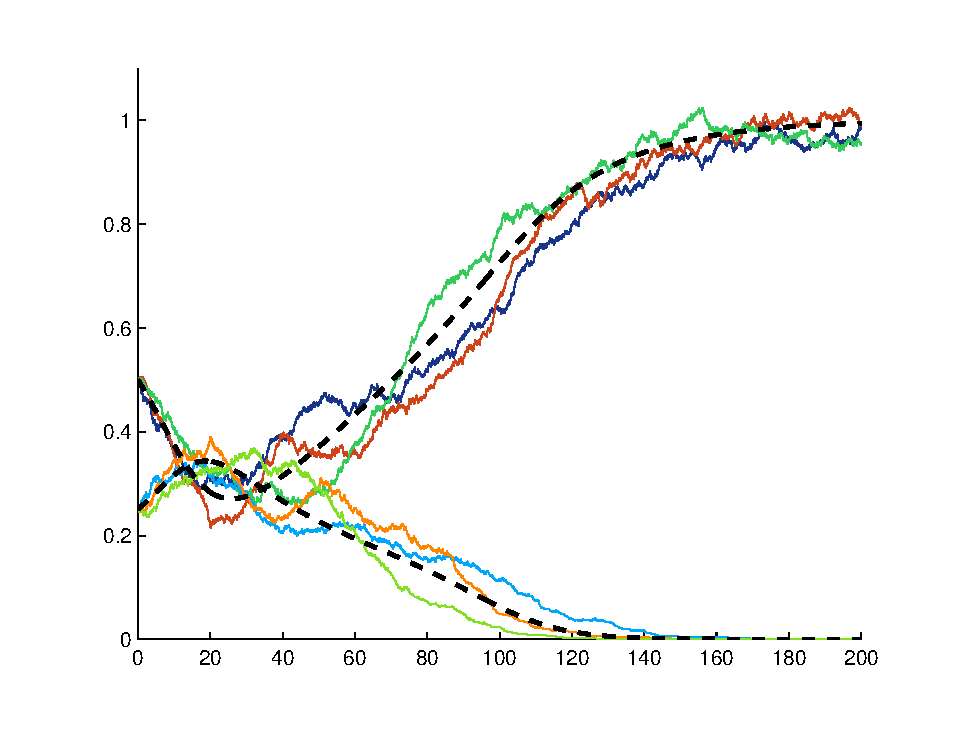
\includegraphics[width=\textwidth]{images/gs_time_evolution.eps}
\caption{Stochastic simulation of the well-stirred Gray-Scott model with $F=0.04$, $\kappa=0.06$, $\rho_s = 2.0$, $u_0=500$ and $v_0=250$. The concentrations ($\Omega=1000$) of both species over times ($t\in[0,200]$)is plotted. Color codeing: dark colors represent species U, bright colors represent species V.}
\label{fig:gs_time_evolution}
\end{figure}

\begin{figure}
\centering
\includegraphics[width=\textwidth]{images/gs_hist_10.eps}
\caption{Histogram obtained by 100000 Gillespie SSA samples evaluated at $t=10$. Parameters and initial conditions similar to figure \ref{fig:gs_time_evolution}}
\label{fig:gs_hist_10}
\end{figure}

\ifdebug
Algorithm (derivation from Oxford Paper)
Leaping condition, tau formula\cite{cao_adaptive_2007}
\begin{itemize}
\item Exact method
\item you can compare time evolution of concentration/number of a specie from deterministic and stochastic simulation 
\item often mean of stochastic realization correspond to deterministic solution, but it is not a rule, but it is nice to show that in the limit of large number of molecules stochastic solution converge to deterministic one
\item A lot of improvements were proposed but it is still computational expensive/prohibitive. 
\end{itemize}
\fi

%\subsection{Tau-leaping Algorithm}
\subsection{Tau-leaping Algorithm}
\ifdebug
Be careful about probability and probability density!!! \\
\fi
The Gillespie Algorithm presented in the previous chapter enables exact numerical simulations of well-stirred chemical reaction systems. It takes account for the inherent randomness in such systems and obeys the same microphysical principles that underlay the Chemical Master Equation. In addition, the algorithm is relatively easy to implement. In practice, however, it turns that even for moderately-sized systems the computational costs of applying the Gillespie algorithm are prohibitive. This is especially true for real-world applications where not just one single trajectory is needed, but a great number of samples must be obtained to estimate probability densities. For every single reaction the system needs to be updated and (some) propensity values have to be recalculated. Consequently, the temporal evolution is obtained up to a level of detail that is neither useful nor necessary for typical applications. It is obvious that there is a need for accelerated (parallelizable) stochastic simulation algorithms. 

In the following, the tau-leaping algorithm originally proposed in \cite{gillespie_approximate_2001} is presented. "By making a minor sacrifices in simulation accuracy, major gains in performance can bet obtained." Considering the overall principle of the algorithm, a clear similarity to the explicit Euler method applied to deterministic models can be observed. 

Equation \eqref{eq:probnot} in the previous chapter gives the probability that a reaction $R_j$ does not fire in an interval $\lbrack t,t+\tau)$. The probability density that it fires in the instant $t+\tau$ is
\begin{align}
f_{1,j}(\tau) = f_{0,j}(\tau) \cdot \alpha_j = \alpha_j \exp(-\alpha_j \tau)
\end{align}
The time one has to wait until reaction $R_j$ fires is therefore exponentially distributed, i.e.\ $\tau \sim \operatorname{Exp}(\alpha_j)$. Without loss of generality, due to the memorylessness of the exponential distribution, i.e.\ $\mathcal{P}(\tau > t + s|\tau > t) = \mathcal{P}(\tau > s)$ the interval $\lbrack0,\tau)$ can be considered. Let $k$ be the number of times the reaction takes place in this interval. Then the probability that $R_j$ fires exactly zeros times is
\begin{align}
\begin{split}
\mathcal{P}(k=0) = \int_\tau^\infty f_{1,j}(t) dt =
\int_\tau^\infty \alpha_j \exp(-\alpha_j t) dt = \exp(-\alpha_j \tau)
\end{split}
\end{align}
The probability that $R_j$ fires exactly once in the interval is
\begin{align}
\begin{split}
\mathcal{P}(k=1) &= \int_0^\tau f_{1,j}(x) \left( \int_{\tau-x}^\infty f_{1,j}(t) dt \right) dx \\
&= \int_0^\tau \alpha_j \exp(-\alpha_j x) \left( \int_{\tau-x}^\infty \alpha_j \exp(-\alpha_j t) dt \right) dx \\
&= \alpha_j \tau \exp(-\alpha_j \tau)
\end{split}
\end{align}
where $x \in \lbrack 0,\tau)$ is the time when $R_j$ actually fires. The inner integral gives the probability that the reaction does not fire thereafter. 

The probability that $R_j$ fires exactly twice in the interval is 
\begin{align}
\begin{split}
\mathcal{P}(k=2) &= \int_0^\tau f_{1,j}(x) \left( \int_x^\tau f_{j,1}(y) \left( \int_{\tau-x-y}^\infty f_{1,j}(t)dt \right) dy \right) dx \\
&= \frac{(\alpha_j \tau)^2}{2} \exp(-\alpha_j \tau)
\end{split}
\end{align}
It can be shown that for arbitrary $l \in \mathbb{N}_0$ the following formula for the probability of counting exactly $l$ firings in the interval is (cite Grimmett, pg. 247, 248)
\begin{align}
\mathcal{P}(k=l) = \frac{(\alpha_j \tau)^l}{l!} \exp(-\alpha_j \tau)
\end{align}
The number of times reaction $R_j$ takes place in the interval $\lbrack 0,\tau)$ is therefore Poisson distributed, i.e.\ $l \sim \operatorname{Pois}(\alpha_j \tau)$. This result is the main idea used in the tau-leaping algorithm. 

Up to now, the implicit assumption that $\alpha \ne \alpha(\vec{x}(t))$ was made. Reconsidering equation \eqref{eq:propensity}, this is not the case. After each firing of a reaction the state changes and so do (in general) the propensities. For the tau-leaping algorithm, however, the assumption is made that the propensities remain approximately constant during a time interval of length $\tau$. Mathematically this can be formulated as follows:
\begin{align}
\abs{\alpha_j(\vec{x}(t+\tau)) - \alpha_j(\vec{x}(t))} \leq \epsilon \alpha_0(\vec{x}(t))
\end{align}
where $0 < \epsilon \ll 1$ is a parameter defined by the user to control model accuracy.  

If this so-called Leap Condition (cite Gillespie) is satisfied, the number of firings for each of the $M$ reactions can be approximated by a Poisson random variable with mean $\alpha_j \tau$. The state of the system at time $t + \tau$ is
\begin{align}
\vec{x}(t+\tau) = \vec{x}(t) + \sum_{j=1}^M k_j \vec{\nu}_j
\end{align}
where $k_j \sim \operatorname{Pois}(\alpha_j \tau)$.

The task of finding a suitable $\tau$, however, is nontrivial. A time step that is too long makes the simulation inaccurate, one that is too short increases computing time. Over the years a variety of different procedures have been proposed (cite some). One of the most sophisticated $\tau$-selection formulas is described in (Cao et al. from R-leap). It is given as follows:
\begin{align}
\label{eq:tau}
\tau = \min\left\{ \frac{\max \left\{ \frac{\epsilon x_i(t)}{g_i}, 1\right\}}{\abs{\mu_i(\vec{x}}}, 
\frac{\max \left\{ \frac{\epsilon x_i(t)}{g_i}, 1 \right\}^2}{\abs{\sigma_i^2(\vec{x}}} \right\}
\end{align}
where $I_{rs}$ is the set of all reactant species in the system. For these species the parameter $g_i$ is defined as follows:
\begin{align}
g_i = h_i + \frac{h_i}{n_i} \sum_{j=1}^{n_i-1} \frac{j}{x_i(t) - j}
\end{align}
$h_i$ denotes the highest order of reaction in which species $X_i$ appears as a reactant, $n_i$ is the number of $X_i$ molecules that are consumed in any of the highest order reactions (Check with 19 of R-leaping paper). The terms $\mu_i$ and $\sigma_i^2$ are given by 
\ifdebug
(What do $\mu$ and $\sigma$ mean?)
\fi
\begin{gather}
\mu_i(\vec{x}) = \sum_{j=1}^M \nu_{ij} \alpha_j(\vec{x}) \\
\sigma_i^2(\vec{x}) = \sum_{j=1}^M \nu_{ij}^2 \alpha_j(\vec{x})
\end{gather}

\paragraph{Remark: Negative populations}
Due to the unboundedness of the Poisson distribution, it can happen that in a leaping step more molecules are consumed than there are available in the system. The resulting negative population of the species is unphysical since the system cannot be in such a state in reality. A lot of different measures to avoid this problem have been proposed (e.g.\ \cite{cao_avoiding_2005, anderson_incorporating_2008}). For this thesis, however, the simplest resolution strategy is chosen: A step which creates negative populations is rejected, the proposed tau is reduced, e.g.\ $\tau_{new} = \tau_{old} / 2$. 
\newpage

The tau-leaping algorithm can be outlined as follows: 

\begin{framed}
\begin{algorithm}[H]
\DontPrintSemicolon
\KwIn{Initial state $\vec{x}_0$, propensity functions $\alpha_j$, time $t_{end}$}
\KwOut{State $\vec{x}(t)$ for $t \in \lbrack t,t_{end}\rbrack$}
 \textbf{Initialization:} Set time $t = 0$ and state $\vec{x} = \vec{x}_0$.\;
 \While{$t < t_{end}$}{
  \For{$j = 1$ \KwTo $M$}
  {
  Compute the propensity function $\alpha_j(\vec{x})$.\;
  }
  Compute the time step $\tau$ according to \eqref{eq:tau}.\;
  \For{$j = 1$ \KwTo $M$}
  {
  Generate a random number $k_j \sim \operatorname{Pois}(\alpha_j \tau)$, i.e.\ the number of time reaction $R_j$ fires.\;
  }
  \If{any of the populations would be negative}{
   Set $\tau = \tau / 2$\;
   Continue at the beginning of the loop\;
   }
  Set $\vec{x} = \vec{x} + \sum_{j=1}^M k_j \vec{\nu}_j$.\;
  Set $t = t + \tau$.\;
 }
 \caption{Tau-leaping Algorithm}
\end{algorithm}
\end{framed}

By leaping over a different time slots instead of considering every individual reaction the computational effort of stochastic simulations can be reduced significantly. The losses in simulation accuracy must be considered, but usually remain within a tolerable range. In the next chapter parallel implementations for multi-core CPU and GPU of the tau-leaping algorithm derived above will be presented. 

\mbox{\color{red}{solve gray-scott and compare to SSA}}

\ifdebug
\begin{itemize}
\item Exact since they generate statistically exact sample paths. Typically, one generates many sample paths (Ausprägungen) to approximate the underlying probability distribution of the system of interest. 
\item But this doesn't work for most systems, since it is computationally too expensive. 
\item Although progress has been made, an exact procedure that simulates every reaction is too inefficient for most realistic problems. 
\item One large population blocks simulation, stiffness, timescales, doesn't influence dynamics of system

\item Approximate method: Major gains in simulation speed obtained by minor sacrifices in simulation accuracy. 
\item Outperforms SSA: Several reactions per step
\item Assumption: Propensity functions $\alpha_k(X(t))$ are relatively constant in a short time interval $(t,t+\tau)$. 
\item Similar to explicit Euler method. Natural connection between SSA in stochastic regime and explicit Euler method applied to the chemical Langevin equation. 
\item Question: How to select the tau?
\item If time-step is too small, then use explicit SSA (Gillespie)
\item Problem: Negative populations --> Solutions proposed in ...
\item How to avoid? R-leaping, SSA for critical reactions
\item Stiffness: Presence of multiple timescales in the system
\item you can plot histogram (pdf for a number of molecules of some specie at some fix time) for different values of parameter epsilon and compare them with histogram from Gillespie
\item this shows what is the role of epsilon
\item To do it, use some non-stiff system, otherwise gillespie will be too slow. E.g. you can use decaying dimerization with non stiff coefficient, or I can give you some other example if you want. Or use the Gray-Scott without diffusion, since it is the illustrative model
\end{itemize}
\fi

\subsection{Parameter Rescaling}
\label{ch:scaling}
The scaling constant $\Omega$ introduced in chapter \ref{ch:def_stoch} gives the number of molecules per volume unit associated with unit concentration in the deterministic model. It can also be though of as the fixed subvolume in the complete domain within which the molecules can move. Concentration is then defined as 
\begin{align}
c = \frac{x}{\Omega}
\end{align}
for $x$ molecules of species $X$. In chemistry, the product of Avogadro's constant $N_A = \unit[6.022 \cdot 10^{23}]{mol^{-1}}$ and a fixed volume of unit size (e.g.\ 1l) is often used as a value for $\Omega$. This, however, is mainly a historic convention and in general, $\Omega$ can be any arbitrary value $\omega > 0$. 

The concept of concentration by definition only makes sense for a macroscopic description of a system. It gives the average number of particles in a fixed control volume. For a system that fulfills the continuum assumption, i.e.\ one for which a macroscopic description is a valid approximation to the microscopic, particle-based reality, the concentration $c(\vec{x})$ at a point $\vec{x}$ in the system barely depends on the chosen control volume containing $\vec{x}$. For small values of $\Omega$, the continuum assumption is violated. In this case the presented deterministic methods are not applicable. If, on the other hand, the number of molecules in a system is large compared to is volume (i.e. $\Omega = \gtrsim 1000$), it can be shown that the deterministic approach based on concentrations and the stochastic approach considering the interaction of individual particles converge \cite{gillespie_deterministic_2009}. This result will be used in chapter \ref{ch:validation} to validate the stochastic simulation tools presented in this thesis by comparing them to the deterministic analytic solutions of several model problems. 

In order to ensure that both, the deterministic and the stochastic model describe the same system, the reaction rates have to be rescaled. The autocatalytic conversion reaction \eqref{eq:r4}, for example, is represented in the deterministic model by the term $\rho_d u v^2$. In the stochastic case, the propensity function of the reaction is $\alpha_4 = \rho_{s} u v (v-1) / (2 \Omega^2)$. For both description to be equal, the relation $\rho_s = 2 \rho_d$ has to hold. For the choice of parameters in this thesis one has $\rho_d = 1.0$ and $\rho_s = 2.0$.

\ifdebug
Alternatives: you can briefly mention R-leaping (just main idea, no need to give all details since we do not use it), and then say that we focus on tau-leaping because sampling in tau-leaping is independent so it can be done in parallel

Compartment approach towards diffusion: Generalization: No every molecule can react with every other molecule, but only within subvolume. \\ you can use some sketch to explain how it works :) The volume of the system is subdivided into a set of uniform subvolumes with spacing lambda. Reactions occur only between molecules within a subvolume $\rightarrow$ CME.
\fi

%\subsection{Compartment-based Stochastic Simulation of Diffusion}
\subsection{Compartment-based Stochastic Simulation of Diffusion}
\label{stochdiff}
To simulate spatially inhomogeneous chemical systems, the concept of compartments has to be introduced. A compartment $c$ is a subvolume of the the complete domain of interest $V$. The set of all compartments $C$ is a partition of the system domain, i.e.\ $c \cap d = \emptyset \:\forall c,d \in C, c \ne d$ (Compartments don't overlap) and $\bigcup_{c \in C} c = V$ (The complete domain is covered by the compartments). The assumption that only particles close to one another can collide and consequently react is reflected by the principle that only molecules within a compartment can interact. Diffusion, on the other hand, is modeled as a jump process of molecules migrating from a compartment to one of its neighbours. Figure \ref{fig:jumpprocess} illustrates the idea. 

\begin{figure}
\centering
\includegraphics[width=\textwidth]{images/jumpprocess.pdf}
\caption{Illustration of the jump process used to model diffusion in stochastic simulations. The front compartment is omitted for reasons of visual clarity. The arrows indicate two out of six possible directions in which the particle can move. }
\label{fig:jumpprocess}
\end{figure}

In general, the shape of the compartments is arbitrary. In this thesis, however, a cubic domain $\lbrack0,1\rbrack^3$ will be decomposed into $L^3$ uniform cubes with side length $h = 1 / L$. Every compartment is identified by its set of indices $(i,j,k) \in [1,\ldots,L]^3$. The volume in space that is covered by the compartment is $\lbrack (i-1)h,ih\rbrack \times \lbrack (j-1)h,jh \rbrack \times \lbrack (k-1)h,kh \rbrack$. 
By introducing stochastic diffusion constants $d_U$ and $d_V$ a modified description of the Gray-Scott model presented in chapter 2 can be obtained:

\underline{Reactions}
\begin{align}
\label{eq:r1mod}
\cee{\emptyset{} &->[F] U_{i,j,k}} \\
\label{eq:r2mod}
\cee{U_{i,j,k} &->[F] \emptyset} \\
\label{eq:r3mod}
\cee{V_{i,j,k} &->[F+\kappa] \emptyset} \\
\label{eq:r4mod}
\cee{U_{i,j,k} + 2V_{i,j,k} &->[\rho] 3V_{i,j,k}}
\end{align}
with positive reaction rate constants $F$, $\kappa$ and $\rho$.

\underline{Diffusion}
\begin{align}
\label{eq:d1}
\cee{S_{i,j,k} &<->[d_S] S_{i\pm{}1,j,k}} \\
\cee{S_{i,j,k} &<->[d_S] S_{i,j\pm{}1,k}} \\
\cee{S_{i,j,k} &<->[d_S] S_{i,j,k\pm{}1}}
\label{eq:d3}
\end{align}
for the two species $\text{S} \in \{\text{U, V}\}$ with positive diffusion constants $d_\text{U}$ and $d_\text{V}$. The spatial dependency of the system is therefore reflected by the compartment index (i,j,k). It is assumed that only particles within a compartment can  react according to equations \eqref{eq:r1mod} - \eqref{eq:r4mod}. Equations \eqref{eq:d1} - \eqref{eq:d3} describe how particles can migrate from one compartment to another. 

It shall be noted that the chosen discretization approach introduces artificial anisotropy to the system in the sense that the number of directions a particle can move in is not infinite, but limited to 6. Consider, for example, a particle that moves along the vector $\lbrack h,h,0 \rbrack^T$. In reality, the distance the particle travels is $d_r = \sqrt{2}h$, in the discretized model it has to travel $d_d = 2h$. For small $h$, however, this effect can be neglected. Furthermore, the analysis of the possible consequences is beyond the scope of this thesis. 

In order to be able to compare the results of the deterministic and the stochastic approach towards diffusion, it remains to derive a relation between the diffusion parameters in both types of simulation. It is obvious that when the compartment length $h$ is reduced, the diffusion constant has to be increased to keep the "average diffusion velocity" of the particles constant. It has been shown (cite) that deterministic and stochastic simulation are equivalent when $d$ is chosen as
\begin{align}
\label{eq:rescale_diff}
d = \frac{D}{h^2}
\end{align}
An illustrative way to derive this relation is as follows: Considering Fick's law of diffusion $\frac{\partial u}{\partial t} = \Delta u$ and applying a central finite-difference approximation for the Laplace operator leads to:
\begin{equation}
\begin{split}
\Delta u &\approx D\frac{u_{i+1,j,k} + u_{i-1,j,k} + u_{i,j+1,k} + u_{i,j-1,k} + u_{i,j,k+1} + u_{i,j,k-1} - 6u_{i,j,k}}{h^2} \\
&= \frac{D}{h^2}u_{i+1,j,k} + \frac{D}{h^2}u_{i-1,j,k} + \frac{D}{h^2}u_{i,j+1,k} + \frac{D}{h^2}u_{i,j-1,k} + \frac{D}{h^2}u_{i,j,k+1} + \frac{D}{h^2}u_{i,j,k-1} \\
&- 6\frac{D}{h^2}u_{i,j,k}
\end{split}
\end{equation}
It is obvious that this is equivalent to the stochastic approach if $d$ is chosen as in equation \eqref{eq:rescale_diff}. 

Considering the results stated above, it turns out that spatially inhomogeneous systems can be simulated with both the Gillespie and the tau-leaping algorithm without any changes just by applying the compartment approach. However, the resulting system is by far more complex than its spatially homogeneous equivalent (in both, a mathematical and a computational sense). Considering $L^3$ cubic compartments in a three-dimensional cubic domain and a reaction system that consists of $N$ local species subject to $M$ reactions, one has $N L^3$ species and $(M+3N) L^3$ reactions. 

\ifdebug
Reasoning: Molecules must collide before they can react (for 2nd and higher order). $\rightarrow$ reaction within compartment makes sure that molecules are close to each other (have a chance to collide)
\fi
\chapter{Stochastic Simulations on Parallel Platforms}
\chapterprecishere{"The way the processor industry is going, is to add more and more cores, but nobody knows how to program those things. I mean, two, yeah; four, not really; eight, forget it."}{\hfill -- Steve Jobs \cite{clarke_ten_2011}}

In accordance with Moore's law exponential growth in the level of integration of microprocessors has been observed for more than five decades. As briefly discussed in the introduction to this thesis this does not necessarily imply equal growth rates in processor performance. In order to harness the enormous raw computing power of modern architectures, it is necessary to develop parallel applications. 

In this chapter two different parallel platforms are presented that are used to enable accelerated implementations of the tau-leaping algorithm. At first a general overview about features, differences and similarities of both platforms is given. Subsequently a more detailed account on ideas, considerations and techniques incorporated into the final implementation follows. 

A lot of research about stochastic simulation algorithms on various parallel platforms has been done in the recent years. Selected examples include \cite{tian_parallel_2005} (OpenMP), \cite{kent_condor-copasi:_2012}, \cite{burrage_compute-intensive_2005} (distributed memory cluster), \cite{macchiarulo_massively_2008} (FPGA) and \cite{nobile_cutauleaping:_2014, li_efficient_2010, klingbeil_stochsimgpu:_2011, vigelius_accelerating_2011} (GPGPU). Depending on application, platform and algorithm significant speedups could be achieved. A novelty of the simulator presented in this thesis is - to the extent of the author's knowledge - the exclusively stochastic handling of diffusion in combination with the tau-leaping algorithm in an approach based on  data parallelism. 

%Burrage K, Burrage P, Hamilton N, Tian T (2006) Compute-intensive simulations for cellular models. In: Parallel Computing for Bioinformatics and Computational Biology: Models, Enabling Technologies, and Case Studies. pp. 79–119.

%\section{GPGPU}
\section{GPGPU}
A Graphics Processing Unit (GPU) is traditionally considered to be an integral part of a workstation computer mainly because it enables accelerated or even real-time rendering of three-dimensional computer graphics. As such, the device relies on a highly specialized and massively parallel architecture. Within a single second hundreds of millions of geometric operations (i.e.\ translation, rotation, scaling) and rendering procedures (i.e.\ interpolation, shading) are applied independently to the polygon primitives of a model by the numerous streaming microprocessors the GPU consists of. Due to the application specific design and since almost all parts of the rendering pipeline are hardware-accelerated, i.e.\ functionality is directly implemented in the physical circuit layout, throughput and computing performance of GPUs are orders of magnitude larger than what a common Central Processing Unit (CPU) can achieve for the same computation. Figures \ref{fig:peakperf} and \ref{fig:memorybandw} show the theoretical peak performance and the memory-bandwidth of selected CPU and GPU models over time. 

\begin{figure}
\centering
\includegraphics[width=\textwidth, trim = 0mm 0mm 0mm 10mm, clip]{images/floating-point-operations-per-second.png}
\caption{Theoretical peek performance of selected Intel CPU and Nvidia GPU models measured in Giga-Floating-point Operations Per Second (GFLOP/s). Image by Nvidia (cite!)}
\label{fig:peakperf}
\end{figure}

\begin{figure}
\centering
\includegraphics[width=\textwidth, trim = 0mm 0mm 0mm 10mm, clip]{images/memory-bandwidth.png}
\caption{Memory bandwidth of selected Intel CPU and Nvidia GPU architectures measured in Gigabytes Per Second (GB/s). Image by Nvidia (cite!)}
\label{fig:memorybandw}
\end{figure}

In order to benefit from this enormous computational power, research has been conducted to investigate if GPUs can be used to accelerate computations beyond the intended scope \cite{harris_physically-based_2002, owens_gpus_2004}. Since the application programming interface (API) of the devices only supported computer graphics development in these days and due to the fact that a lot of the functionality on the device is hardwired, a general problem has to expressed in terms of pixels, textures and shaders. This process requires a lot of experience, detailed knowledge about the hardware and computer graphics programming as well as trial and error optimization. Apart from these practical hurdles, it turned out that a lot of parallel algorithms, i.e.\ algorithms that consist of independent subproblems that are processed in parallel, can outperform an equivalent CPU implementation by orders of magnitude. 

The term General Purpose Computation on Graphics Processing Unit (GPGPU) was coined by Mark Harris in 2006 \cite{luebke_gpgpu:_2006}. At around the same time, GPU manufacturers realized that scientific computing might be a new market for their products. However, in order to enable the average researcher to harness the computing horsepower of the GPU, improvements in both hardware and software had to be made:
\begin{description}
\item[Hardware] Over the course of subsequent GPU generations, the flexibility as well as the programmability of the streaming multiprocessors (also called shading units or shader) has increased. Furthermore, essential primitives for concurrent programming such as synchronization and atomics were introduced and optimized. In addition, standard CPU features that were formally not available on GPUs like an automatically managed cache or double-precision floating-point arithmetic were added. Both major vendors of GPUs, AMD and Nvidia, have introduced special versions of their devices for professional high performance computing (HPC) applications. Those products, branded AMD FireStream and Nvidia Tesla, respectively, are optimized for use in multi-GPU cluster located in computing centers. 
\item[Software] At an even faster rate than hardware improvements, software innovations were presented. At first, native development in widely-known high-level languages such as C or C++ was enabled\footnote{The language dialect used for GPU development is usually not absolutely compliant with the original standard language. On the one hand some minor language features are sometimes ommited (i.e.\ CUDA-C does not support function pointers), on the other hand small additions are added to account for GPU-specific features and properties.}, later bindings for Python, Java, MATLAB and others were provided. In a next step, highly optimized compilers, debuggers, performance analysis tools and complete integrated development environments (IDE) were shipped to further improve development efficiency and product performance. Furthermore, libraries for applications such as linear algebra (BLAS, SPBLAS), signal processing (FFT) and random number generation were introduced. Now, an existing application can be accelerated just by replacing the library used, without writing a single line of GPU code. 
\end{description}

Over the years, several programming frameworks and standards for GPGPU were introduced. In the following a short overview is given.  
\begin{description}
\item[OpenCL] The Open Computing Language is an open standard for computation on heterogeneous platforms. As such, it can not only be used for GPU programming, but also to create applications that make use of systems that consist of numerous CPUs and so-called accelerators\footnote{Field Programmable Gate Array (FPGA), Digital signal processor (DSP), GPU}. It is based on the C/C++ programming language. The standard has been adapted by over 30 companies, including AMD, Intel and Nvidia. OpenCL 1.0 was introduced in December 2008, the latest version OpenCL 2.0 published in November 2013 includes novel execution models and introduces features of C++11. (cite)
\item[OpenACC] The Open Accelerators standard is developed by several companies including Cray, Nvidia and PGI. OpenACC is conceptually similar to the widely-used Open Multi-Processing (OpenMP) standard for parallel programming in shared memory systems (see chapter ??). The framework primarily consists of a set of compiler directives that can be used to mark regions that are to be run on an accelerator device. The main advantage of this approach is that the developer does not need to know the details of a potentially complicated framework, but can still significantly improve the performance of existing code just by adding compiler directives. Version 2.0a of the standard was ratified in August 2013. 
\item[CUDA] The Compute Unified Device Architecture is a proprietary framework developed by Nvidia. An initial beta version was published in February 2007. Due to its widespread and early distribution on the market and the large number of libraries, tools and resources available, CUDA is considered to be the marking leader for GPU computation. The GPU implementation of the tau-leaping algorithm presented in this thesis is based on CUDA. The most recent version, CUDA 6.0, was published in April 2014. It provides a unified view on CPU and GPU memory and improved scaling for multi-GPU systems. In the following section more detailed information on the paradigms and features of CUDA will be given. 
\end{description}

\ifdebug
\begin{itemize}
\item General-Purpose computation on Graphics Processing Units
\item GPGPU allows the developer to exploit the great computational power of modern GPU by giving access to the underlying parallel architecture that was conceived for speeding up real-time three-dimensional computer-graphics. (Nobile)
\item What is the difference between CPU and GPU
\item Trends
\item What kind of problems are suited for GPU?
\item Modern GPU are throughput-orientated devices with massively parallel architecture. The model used for the simulations ... TFLOPS. 
\item Avoid branches
\end{itemize}
\fi

\subsection{Nvidia CUDA} \label{ch:cuda}
The Nvidia CUDA computing platform combines two major paradigms of modern data processing devices: \textit{Single Instruction, Multiple Data} (SIMD) and \textit{multi-threading}. Following the data parallelism approach, the former principle describes the ability of a processor to apply the same operation to different pieces of data at once. The later, on the other hand, distributes independent instruction streams (\textit{threads}) to the available processors. 

The abstract principles mentioned above can be derived directly from the actual hardware architecture of the device: A Nvidia GPU consists of an array of \textit{Streaming Multiprocessors} (SM) which in turn are formed by a number of so-called \textit{CUDA-cores}. Following the SIMD principle, a SM can only execute one instruction at a time, i.e.\ all cores have to apply the same operation to their current data point. If there is code branching within the instructions issued to one SM, individual cores may skip the operations of a non-applicable branch. This leads to serialization of the execution so that in general branching should be avoided whenever possible. 

Within the instruction stream running on a SM data parallelism is expressed using the SIMD principle. On a larger scale, considering only the multiprocessor units and their in general different instruction streams, task parallelism can be observed. Analogous to the cores within a conventional CPU, all SMs execute at the same time and so do the threads running on them. On Nvidia GPUs, however, communication and synchronization between threads is limited. 

From the point of view of a software developer, a CUDA program consists of code for the host (i.e.\ the CPU) and the device (i.e.\ the GPU). Device procedures, so-called \textit{kernels}, must be launched in the host section of the application. The kernel is then automatically replicated many times to create individual threads. In CUDA, threads are organized in one-, two- or three-dimensional structures called \textit{blocks}, which in turn are part of a \textit{grid}. The size of a block is limited by the hardware and so is the size of blocks and grids. Threads within a block can be synchronized during execution of the kernel, on a global level, however, the only way of synchronizing all threads is the invocation of two destinct kernels. The device assigns blocks to SMs and further splits them to form batches of 32 threads named \textit{warp}. Since the number of threads per warp is equal to the number of cores per SM, a warp can be executed directly. Each thread can determine its position in grid, block and warp at runtime. The complex dispatch and scheduling procedure allows CUDA programs to achieve good performance on different GPUs independent of the properties of the specific model (e.g.\ number of SMs). Figure \ref{fig:cuda_threads} visualizes the concepts introduced above. 

\begin{figure}
\centering
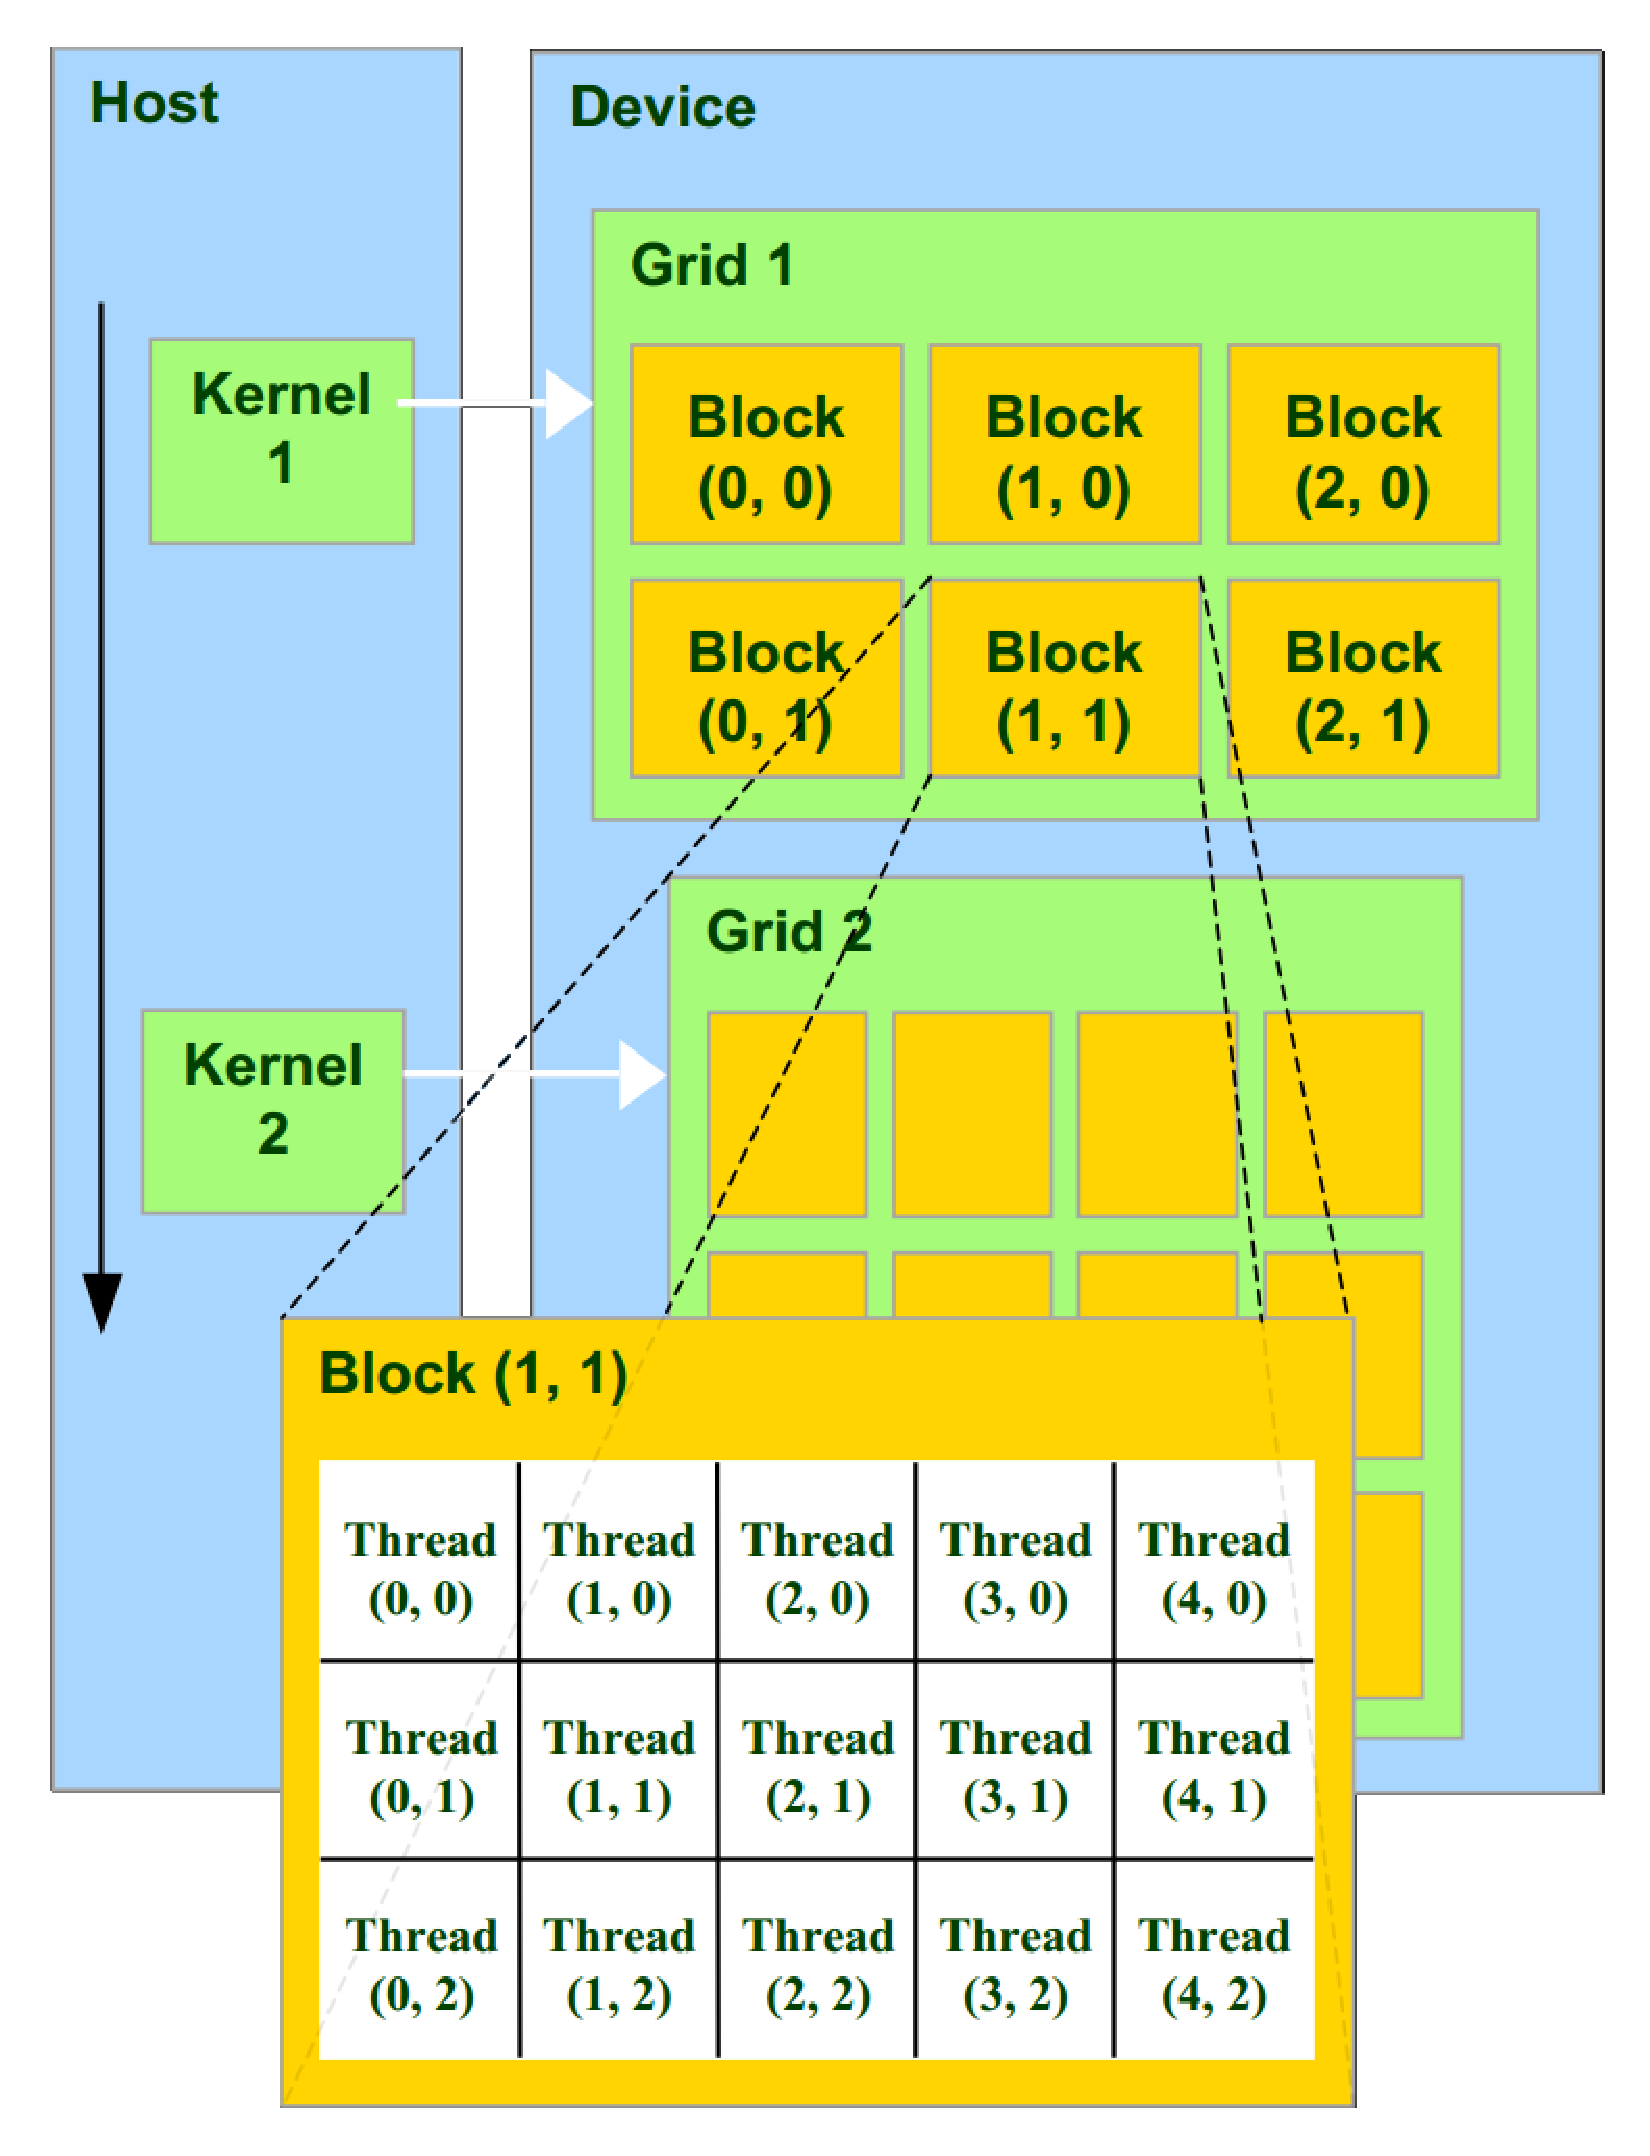
\includegraphics[height=10.0cm]{images/cuda_threads.eps}
\caption{Illustration of the CUDA programming model. Figure taken from \cite{nvidia_cuda_2012}.}
\label{fig:cuda_threads}
\end{figure}

One of the most important aspects to consider when developing GPU applications is the memory hierarchy of the device. Figure \ref{fig:memoryhier} gives an overview over that different kinds of memory on the device, table \ref{tab:bwandaccess} lists bandwidth and latency. 
\begin{description}
\item[Global memory] Global memory can be considered to be the GPU equivalent of the CPU main memory. Its capacity usually exceeds several gigabytes, the bandwidth is in the order of 100 GB/s (see figure \ref{fig:memorybandw}). It is the only kind of memory that can be accessed directly from the host CPU via the PCI-Express port ($\sim$6 GB/s). (some additional sentences)
\item[Shared memory] Data in shared memory is private per thread-block, i.e.\ it can only be accessed by the threads in a block for data exchange. After the complete block has finished execution, its data in shared memory cannot be accessed any more. Physically shared memory is located in banks close to the individual SMs. The bandwidth is usually around 7-10x faster than global memory bandwidth. Since accessing the latter often limits the overall performance of a CUDA application, shared memory can help to reduce the number of expensive global memory transactions by keeping data that is used more than once close to the SM (spatial locality). It is often considered to be a programmer-managed L1 cache. In fact, modern GPUs have an automatically managed L1 cache which physically shares its banks with the latter.  (cite cuda handbook, kaufmann)
\item[Registers] One of the main difference between GPUs and CPUs is the number of registers available. Registers are small but extremely fast memory units that usually only store one single value. They are located very close to the processor such that its content can be fetched almost instantly (i.e.\ within a single clock cycle). A standard multi-core CPU performs best if it can execute a small number of threads in parallel. If the number of threads occupying the processor grows, the overall performance decreases since frequent context switches are needed to ensure that every thread gets a fair share of the computing power. In this process it is necessary to restore the state of a suspended thread before it can execute again, i.e.\ the register values of the previously active thread have to be stored and those of the next thread have to be restored. On a CPU, this is a length process, but on a GPU ever thread has its own set of registers so that context switching does not involve refilling registers with values stored in slower memory regions. Fast context switching can therefore be used to hide memory latencies: Whenever a warp stalls because it has to wait for a memory transaction to finish, another warp can be executed. The delay of this switch is negligible. 
\end{description}
For the sake of completeness it has to be mentioned that there are other kinds of memory (e.g. constant and texture memory) that can be accessed in CUDA. They can be useful for some applications, especially for image processing tasks, but are of no great use for the application presented in chapter \ref{ch:gpuimplementation}. 

Furthermore, it is important to note that registers and shared memory have to be considered precious resources in CUDA development. Writing, for example, a kernel that uses to many registers limits the number of blocks that can reside simultaneously on a SM. This, in turn, reduces the number of warps that are available for execution. If there are no alternatives for the processor available to choose from when one warp stalls, the latency of the memory access cannot be hidden. 

\begin{table}
\centering
\begin{tabular}{|l|l|p{2.8cm}|l|}
\hline
 \textbf{Storage Type} & Registers & \mbox{Shared Memory} L1 Cache & Global Memory \\ \hline
 \textbf{Bandwidth} & $\sim$8 TB/s & $\sim$11.5 TB/s & $\sim$200 GB/s\\ \hline
 \textbf{Latency} & 1 cycle & 1-32 cycles & 400-600 cycles \\ \hline
\end{tabular}
\caption{Bandwidth and access time by memory time (Adapted from \cite {cook_cuda_2012}, fixed)}
\label{tab:bwandaccess}
\end{table}

%http://www.sdsc.edu/us/training/assets/docs/NVIDIA-02-BasicsOfCUDA.pdf
\begin{figure}
\centering
\includegraphics[width=\textwidth]{images/gpuarchitecture.pdf}%memory-hierarchy.png
\caption{The memory hierarchy of Nvidia GPUs (simplified view, adapted from \cite{nvidia_cuda_2012}}
\label{fig:memoryhier}
\end{figure}

\ifdebug
\begin{itemize}
\item History
\item Memory model (important since "computation is for free"
\item Libraries (cuRAND, Thrust) (It's hard to get it right $\rightarrow$ use them)
\item Cross-platform GPGPU library that combined SIMD and multi-threading. Branches should be avoided. 
\item Developer implements kernel, a C function that is loaded from the host (the CPU) to the device (the GPU). It is replicated in many copies named threads. Threads can be organized in three-dimensional structures named blocks which, in turn are part of a grid. 
\item Whenever the host calls a kernel, the device automatically creates the corresponding grid and schedules each block on one streaming multiprocessor (SM) available on the GPU. 
\item Hardware constraints: Block size, registers, blocks per SM, shared memory, ...
\item Warp: 32 threads
\item Memory: shard, global, registers, ... Go beyond the scope of this thesis. 
\item Goal: Have enough memory transactions in flight to hide latency
\end{itemize}
\fi

\subsection{Implementation}
\label{ch:gpuimplementation}
In this chapter the tau-leaping simulator developed in the context of the thesis will be presented. At first, general execution steps of the program and implementation details are discussed. Afterwards, some of the main ideas that were incorporated into the application are explained in more detail. This chapter is solely explanatory in character, the results of numerical validation and performance evaluation experiments will be presented in chapter~4. 

Algorithm \ref{alg:pseudogpu} gives a pseudocode description of the GPU implementation of the tau-leaping algorithm developed for this thesis. Considering the Gray-Scott model as the primary example of this work, the description below represents the special case for $N = 2$ species. It can, however, easily be generalized. In the following the central parts of the implementation are presented in more detail. 

\begin{enumerate}
\item \textbf{Initialization:} During the initialization stage of the application memory for the simulation state is reserved. On the device, two arrays of datatype Integer (int) are reserved to store the number of particles of each species. In the concrete example the arrays are named \texttt{d\_X1a}, \texttt{d\_X1b}, \texttt{d\_X2a} and \texttt{d\_X2b} where \texttt{X1} and \texttt{X2} represent species U and V, respectively. The size of the arrays depends on the number of compartments the system consists of. For example, if the cubic domain of a system is divided into 128x128x128 subvolumes (and assuming \texttt{sizeof(int) = 4}), one array occupies 8 MB of global memory space. To allow parallel execution of the algorithm, two fields for every species are needed to store the previous and the modified state of the system. Furthermore, if negative populations are observed after a leaping step, the old state can easily be reverted. 

Furthermore, two additional arrays have to be allocated on the GPU: \texttt{d\_states} and \texttt{d\_tau\_per\_cell}. The former is used to store the state structures of the pseudo random generators used in the simulation. For the choice presented in the next section, the maximum size is 48 Byte times the number of compartments. The latter is an integral part of the procedure to calculate the leap-length $\tau$ according to equation~\eqref{eq:tau}. Its size depends on the number of CUDA-blocks spawned on the device during the simulation, it contains floating point numbers, i.e.\ \texttt{float} in the given example. The array contains the minimum value derived from the state of the individual compartments of a block. To determine the value of $\tau$ that is used for the next simulation step, the minimum of the values in the array has to be found. A more detailed explanation of the procedure is given in part \ref{enum:4} of this enumeration. 

After being allocated, the values of the device arrays are set by invocating an initialization kernel. It creates and correctly seeds the PRNG states. In addition, the prescribed initial conditions are evaluated and stored in the species state arrays. 

In order to write the state of the simulation to a file, it is necessary to copy the data from the GPU's global memory to the host main memory. This is the reason why on the host an array of the same size has to be allocated for each species of interest. The prefixes '\texttt{d\_}' and '\texttt{h\_}' are used by convention to distinguish between host and device arrays. To achieve best data transfer performance, it is important to use so-called pinned memory, i.e.\ host-side memory that cannot be swapped out to disk by the operating system so that it is instantly available for Direct Memory Access (DMA) copying. Pinned memory can be allocated by library functions that are part of the CUDA framework. 
\label{enum:init}

\item \textbf{CPU-GPU-interaction:} One of the traditional shortcomings of CUDA and GPU computing in general is the fact that complex control flows cannot be handled on the device. Furthermore, kernels can only be launched by the host, not from within GPU code. For the presented tau-leaping implementation this means that the main simulation loop (\texttt{while t < t\textsubscript{end}}) is run on the CPU. Even though all important computations are done in GPU memory, some values such as the proposed tau value or the information if negative populations have been detected must be transferred to the host. If the whole simulation procedure was be manged by the device itself, a lot of time-consuming communication could be avoided. In practice however, implementing the whole algorithm in one complex kernel would neither help achieve high-performance (due to unavoidable branching) nor would it be possible at all (lack of global synchronization). 

On modern Nvidia devices (compute capability $\geq$ 3.0) a feature called Dynamic Parallelism enable kernel invocation within GPU code. Since the tau-leaping simulator presented in this thesis was developed for previous generation hardware (i.e.\ compute capability 2.0), the feature could not be exploited. However, it seems to be promising and should be considered for future work (see \ref{ch:outlook}). 

\item \textbf{Random number generation:} To imitate the stochastic behaviour of the simulated system, any SSA is highly dependent on availability, quality and performance of random number generators. In practice random number generation is usually the computationally most demanding part of the algorithm. The cuRAND library by Nvidia offers several different pseudo-random number generator implementations that support various statistical distributions. The manufacturer claims that the library can outperform CPU-based solutions on current-generation hardware by a factor of almost two orders of magnitude. In the tau-leaping simulation a great number of Poisson-distributed random numbers with varying mean are needed, a functionality that cuRAND offers since version~5.0. XORWOW \cite{saito_variants_2010} is used as the underlying PRNG since it is a good compromise between performance (i.e.\ gigasamples/second), state size and statistical correctness. 

\item \textbf{Thrust library:} In CUDA, "common and important data parallel primitives [are] easy to implement [, but it is] harder to get it right" (Harris, 2007). To increase developer efficiency as well as application performance, several CUDA libraries have been introduced to provide easy access to highly-optimized algorithms and subroutines. The Thrust library of parallel algorithms \cite{hoberock_thrust:_2010}, for example, is shipped directly with the CUDA toolkit. It closely resembles the C++ Standard Template Library (STL) known to many developers. Its performance in benchmarks as well as in real-world application is considered to be out of reach for the average researcher who uses CUDA for simulations. In the tau-leaping implementation presented in this thesis two operations provided by thrust are of great importance: parallel minimum reduction and predicate-based logical reduction. The former is used to find the minimum value of $\tau$ proposed by the compartments stored in the \texttt{d\_tau\_per\_cell} array (see \ref{enum:init}). The latter, more precisely the function \texttt{thrust::any\_of} together with the unary predicate \texttt{is\_negative} is applied to the modified state arrays of both species X1 and X2. It is used to determine if the proposed step has produced negative molecule populations and, if that is the case, it has to be rejected. 

\item \textbf{Tau Selection Procedure:} \label{enum:4}
A good example of how library functions and custom CUDA-kernels by the developer can go hand in hand is the implementation of the tau-selection procedure according to equation \ref{eq:tau}. In a first step, the values for $g_i$ and $x_i$ can be determined by the individual thread. Due to the spatial dependency in the simulated system introduced by diffusion, to calculate the mean $\mu_i$ and the variance $\sigma_i^2$ it is necessary that the molecule population counts of the neighbouring compartments are known. To reduce the number of expensive accesses to global memory, shared memory is used to exploit the principle of data locality within the three-dimensional blocks. Further on, after every thread has calculated its individual tau value, the block-wise minimum of the proposed values is found via reduction in shared memory. Once the kernel has finished execution, the final value for $\tau$ is determined by the high-performance reduction routines provided by Thrust. 

\item \textbf{Reaction kernel:} Implementing the in-compartment reactions \eqref{eq:r1} - \eqref{eq:r4} is straightforward. In the common framework to classify parallel functions \texttt{kernel\_reactions} implements a map operation. In the concrete example this means that every thread reads two values from distinct positions in two arrays (i.e.\ the molecular population counts of its compartment) and writes two values to distinct positions in two other arrays (i.e.\ the molecular counts after the reactions have fired). The operation does not require any synchronization, nor can GPU resources apart from global memory be used to speed up the computation. 

\item \textbf{Diffusion kernel:} Implementing the diffusion kernel and achieving good performance, on the other hand, is much more difficult. Several different approaches can be taken and features of the underlying hardware can be used to accelerate the computation. In the following the main ideas of three different diffusion kernels will be presented. The results of performance analysis will be presented together with other optimization techniques in chapter \ref{ch:gpuopt}. 
\begin{enumerate}
\item \textbf{diffusion\_naive:} This first approach does not make use of shared memory and relies heavily on atomic operations (also called atomics). At first, every thread loads the population counts of the own and neighbouring compartments from global memory. These accesses are not only redundant (every value is needed by 7 threads in 3D), but also strided due to the layout of the compartments in memory (x is the fastest direction, z the slowest). If a thread with three-dimensional index $(i,j,k)$ needs to access a value at $(i+1,j,k)$ (i.e.\ the neighboring compartment in positive x-direction), it can be found right next to its own value. If, however, $(i,j,k+1)$ is accessed, $L^2$ values are in between. Since memory is always accessed in lines, this will definitely affect performance. Considering, for example, Double Data Rate (DDR) memory and a 384 bit wide memory bus, with every memory transaction 24 integer values can be accessed. If just one value is actually needed, only a small fraction of the theoretical peak bandwidth is used. 
When a thread has fetched all the values it needs, it uses Poisson-distributed random variables to determine how many molecules leave the compartment through the six (2D: 4) faces. These numbers then need to be added to or subtracted from the respective values in the state arrays. These accesses are again strided and atomic operations need to be used to avoid data races. Every position in the array is written to seven times and if two or more threads try to modify the value at the same time, incorrect result may be obtained. 

Even though no performance data will be given in this chapter, it is obvious that this first naive approach leaves a lot of space for improvements. Due to the simplicity of the actual code it is suitable to show correctnes of the algorithm and it can act as a reference for more sophisticated approaches. 
\item \textbf{diffusion\_shared} One obvious way to improve the naive approach is to make use of shared memory. If all population counts belonging to threads in a three-dimensional cubic block are stored locally at the SM, almost 6 out of 7 global memory transactions can be saved. Furthermore, the relative performance of strided access patterns and atomic operations in shared memory is overproportionally good compared to global memory. To ensure that in a first step all necessary values have been loaded, all threads in a block have to be synchronized by a barrier. Afterwards, diffusion can be simulated the same way it was described above, this time in fast shared memory instead of slow global memory. When all those operations have finished, the resulting delta-values (i.e.\ the difference between old and new state) are added to the global memory arrays. Compartments at the outer shell of one block are accessed by threads from at least one neighbour (up to three at the corners) so that atomics are needed to ensure correct results. 

An additional challenge that arises from this approach is question of how to handle accesses to neighbouring compartments that are not part of the same block. The simplest idea to handle 'out-of-block reads' is to just fall back to global memory. Since these values are only needed by one thread, there is no use in storing them in shared memory. For 'out-of-block writes' so-called overflow buffers can be introduced. Whenever a delta-value is supposed to be added to an 'out-of-block' compartment, it is stored in this temporary field. After all threads of the block have finished their computation of diffusion, the overflow buffers are added to global memory together with the regular delta values. 
% improvement: memory access when writing them back
\item \textbf{diffusion\_four}
The main idea of the third approach presented is to avoid atomic operations in global memory altogether. If the pattern of active blocks resembles that of a three-dimensional chessboard, the overflow buffers are written to positions in the state arrays that are not owned by an active thread. It is termed \texttt{diffusion\_four} due to the four distinct kernel launches that are needed for the approach. The pattern of active blocks is illustrated in figure \ref{fig:four}. Apart from a more complicated index calculation section in the beginning, the kernels work exactly the same like the previously presented approach. Avoiding atomic operations comes at the coast of the overhead introduced by three additional kernel launches. 
\end{enumerate}

\begin{figure}
\centering
\includegraphics[width=\textwidth]{images/four.png}
\caption{Illustration of the access pattern of \texttt{kernel\_four}. Red blocks are active. }
\label{fig:four}
\end{figure}

It shall be noted that in practice, since all the data that is needed for \texttt{kernel\_reactions} is available within the diffusion kernel, the two are combined to reduce the number of kernel launches and global memory transactions. 
\item \textbf{Output file:} In order to visualize the temporal evolution of the system over time, it is necessary to save the state of the system to the hard drive disk (HDD) in user-defined intervals. For best performance the arrays are written to files in binary, i.e.\ the sequence of bits in the files and in memory is equal. Whenever the control loop on the host enters the output section, data has to be copied from GPU to CPU memory. Since kernel launches in CUDA are asynchronous and input/output operations are managed by the operating system in the background, the application can continue regular execution even before the file has been stored on the comparably slow HDD. Apart from performance considerations one of the main advantages of the binary file format (.bin, .raw) is that it can be read by almost all programs one may use for post-processing. If that is not the case, data can easily be converted with tools such as MATLAB. On the other hand, it shall be noted that binary files are not necessarily interoperable (e.g. depending on system architecture, operating system and compiler different result may be produced), they are not readable for humans and a lot of implicit information such as data type, endianness, system dimension and coordinate axis ordering has to be provided to be able to work with the file. 
\end{enumerate}

%\begin{mdframed}
\begin{algorithm}[H]
\DontPrintSemicolon
%\KwIn{Initial state $\vec{x}_0$, propensity functions $\alpha_j$, time $t_{end}$}
%\KwOut{State $\vec{x}(t)$ for $t \in \lbrack t,t_{end}\rbrack$ (TODO)}
\textbf{Initialization:} \\
Allocate state arrays $\mathtt{d\_X1a}$, $\mathtt{d\_X1b}$, $\mathtt{d\_X2a}$ and $\mathtt{d\_X2b}$ on the device. \\
Allocate random generator state array $\mathtt{d\_states}$ on the device. \\
Allocate local tau array $\mathtt{d\_tau\_per\_cell}$ on the device. \\
Allocate state arrays $\mathtt{d\_X1}$ and $\mathtt{d\_X2}$ on the host. \\
Execute $\mathtt{kernel\_init\_device(d\_X1a,\ldots,d\_X2b,d\_states)}$. \\
Write initial state to file.\;
\textbf{Simulation loop:}\\
Set pointer $\mathtt{d\_X1\_old} \rightarrow \mathtt{d\_X1a}$. \\
Set pointer $\mathtt{d\_X1\_new} \rightarrow \mathtt{d\_X1b}$.  \\
\ldots\footnote{Analogous for $\mathtt{d\_X2\_old}$ and $\mathtt{d\_X2\_new}$.}\\
\While{$\mathtt{t} < \mathtt{t_{end}}$}{
Execute $\mathtt{kernel\_tau\_local(d\_X1\_old,d\_X2\_old,d\_tau\_per\_cell)}$. \\
Set $\mathtt{tau} = \mathtt{thrust::reduce(d\_tau\_per\_cell,thrust::minimum)}$. \;
\While{$\mathtt{true}$}{
Execute \texttt{kernel\_reactions(d\_X1\_prev,\ldots,tau,d\_states)}. \;
Execute \texttt{kernel\_diffusion(d\_X1\_prev,\ldots,tau,d\_states)}. \;
\eIf{$\mathtt{thrust::any\_of(d\_Xi\_new,is\_negative())}$\footnote{For any of the two arrays $\mathtt{d\_X1\_new}$ and $\mathtt{d\_X2\_new}$, i.e.\ $\mathtt{i} = 1,2$.}}{
$\mathtt{tau} = \mathtt{tau / 2}$\;}{
\texttt{break} \;
}
} %end while true
\If{$\mathtt{t} \geq \mathtt{write\_counter} * \mathtt{write\_every}$ }{Write current state to file.}
Swap $\mathtt{d\_X1\_old}$ and $\mathtt{d\_X1\_old}$. \\
Swap $\mathtt{d\_X2\_old}$ and $\mathtt{d\_X2\_old}$. \;
} % end simulation loop
\textbf{Finalization:} \\
Write final state to file. \\
Deallocate arrays and reset device. \;
\caption{Overview for GPU implementation !!!}
\label{alg:pseudogpu}
\end{algorithm}
%\end{mdframed}

\ifdebug
\begin{itemize}
\item Memory limitation: Large systems may exceed on-board capacity of a single GPU $\rightarrow$ spatial decomposition, communication, load balancing, complicated (cite Hallock)
\item The application was compiled with ... It depends on CUDA 6.0 (released...).
\item Thesis comes with code. Can be used..., warranty, ...
\end{itemize}
\fi
%\section{Multi-core CPU}
\section{Multi-core CPU}
For a long time the main driver of CPU performance growth has been the clock rate. Within the first years of the new millennium, however, it became obvious that this principle could not be exploited for any further progress. For CPU frequencies beyond 3-4 GHz, it is practically impossible to dissipate the heat released in the chip with common CPU coolers, the so-called \textit{power wall} was reached \cite{kuroda_cmos_2001}. In order to enable further performance growth, multi-core architectures were introduced. Instead of trying to improve a single core at enormous expenses, several potentially smaller cores are placed on a single chip. The resulting CPU can then execute several threads truely in parallel, i.e.\ not only just by assigning timeslots to individual threads. The novel approach turned out to be very successful so that the great majority of processors sold nowadays implement a multi-core architecture. 

The downside of this paradigm change from the point of view of a developer is that programs do not automatically execute faster when a new generation of CPUs is introduced. The individual core does not necessarily get any faster and since they are executed one step at a time, sequential programs cannot make use of the increasing number of concurrent computation units in modern chips. 

To allow an application to benefit from the parallel architecture, the developer has to explicitly declare sections that can be run concurrently. In the majority of today's most popular programming languages little to no means of expressing parallelism are provided. Even though this is about to change (C++11 has introduce threads, Java's concurrency package is planned to be given a major overhaul), still a lot of work has to be done in this field. 

In general, there are two different approaches towards enabling concurrency in an application: Using explicit threading subroutines provided by the operating system (OS) or relying on semi-automatic compiler functionality. The former means that the developer has to explicitly create threads, implement scheduling routines and manage synchronization. On Microsoft Windows systems threading is provided as part of the Base Services included in the Windows API, in a Unix-like environment POSIX Threads (Pthreads) can be used. The latter approach is considered to be significantly faster to apply and easier to learn. It is especially useful when already existing legacy code should be parallelized since the structure of the program does not need to be changed significantly. Two of the most commonly used frameworks are Intel Threading Building Blocks (TBB) and the Open Multi-Processing standard (OpenMP). In the back end semi-automatic solutions depend on the native threading routines available on the targeted operating system. Therefore in practice the performance of both approaches is comparable. The additional level of control obtained by explicitly using OS routines comes at the cost of greater development effort. 

\subsection{OpenMP}
"OpenMP is a specification for a set of compiler directives, library routines, and environment variables that can be used to specify high-level parallelism in Fortran and C/C++ programs. \cite{openmp_architecture_review_board_frequently_2014}" A first version for the Fortran programming language was published in October 1997, support for C/C++ was added in October 1998. The latest version, OpenMP 4.0, was released in July 2013. OpenMP (OMP) implements the fork-join multithreading model, i.e.\ there is one master thread which can be forked to create several other threads. A region of parallel execution is ended by joining all threads with the master. To distribute the work available in a parallel region, OpenMP comes with a variety of scheduling strategies such as static (i.e.\ compiletime) and dynamic (i.e.\ runtime) scheduling. Outside of this region the program is executed sequentially. 

Creating a parallel region in OpenMP is straighforward: In C/C++ the directive \texttt{\#pragma omp parallel} orders the compiler to create several threads by forking the master thread. The number of threads can be prescribed by the developer, set at runtime or determined automatically by the system taking into account the number of physical execution units. If a compiler does not know the standard (or the necessary flags to enable it are not set), the directives will be ignored and in most situations a working serial version of the application can be created. 

By default all the code enclosed by the the braces (\{\ldots\}) specifying beginning and end of the parallel region is executed by ever thread. To tell the compiler that a specific subsection should only be executed once, directives such as \texttt{\#pragma omp single} or \texttt{\#pragma omp master} can be used. The work within a for-loop is shared by adding \texttt{\#pragma omp for} in front of it. If the parallel region consist just of a single loop, this can be shortened to \texttt{\#pragma omp parallel for}. Apart from simple loop parallelization OpenMP offers more advanced features such as reduction, atomic operations, explicit thread synchronization and (debuting in version 3.0) tasks. For an in-depth introduction to all the features of OpenMP the reader shall be referred to an online course by Tim Mattson from Intel\footnote{Tim Mattson is one of the original developers of OpenMP. His video lectures can be found online at \url{http://goo.gl/VObNd1}, the complementary slide at \url{http://goo.gl/bDWka6}.}. 

\subsection{Implementation}
In the following the implementation details of the multi-core CPU version of the developed tau-leaping simulator will be presented. The OpenMP standard is used for parallelization. In the pseudocode description given in algorithm \ref{alg:pseudocpu} a lot of conceptual similarities to the GPU implementation (see algorithm \ref{alg:pseudogpu}) can be observed. There are, however, certain differences that directly reflect the differences of the underlying hardware. 

\begin{enumerate}
\item \textbf{Initialization:} Just like in the GPU version, two arrays of type \texttt{int} are used in the algorithm to represent the number of molecules of one species in the individual compartments. For the two species in the Gray-Scott example, these fields are called \texttt{h\_X1a}, \texttt{h\_X1b}, \texttt{h\_X2a} and \texttt{h\_X2b}. Even though all simulation data resides in CPU main memory, the \texttt{h\_} prefix is used to underline the similar structure of both implementations. 

The required reduction operation to find the minimum proposed tau value is a built-in feature of OpenMP (\texttt{\#pragma omp for reduction (min:tau)}) so that there is no need for an additional array to explicitly store candidate values. Furthermore, unlike in the GPU case, no temporary storage for IO operations is needed since data from main memory can be written directly to the HDD. The PRNG states are encapsulated in a helper object of type \texttt{paraRNG}, a class that was developed to enable thread-safe access to a variety of RNG implementations (see section \ref{enum:cpu:rng}). 
\item \textbf{Parallel region:} An important characteristic of the presented algorithm is the fact that there is solely one large parallel region. It may seem counter-intuitive to make all threads deal with the work introduced by evaluating loop control conditions. However, this additional effort is negligible compared to the overhead that would be introduced if threads were continuously created and destroyed. Sections that shall be executed exactly one are guarded by the directive \texttt{\#pragma omp single}. Unlike in the CUDA implementation where separate kernel invocations are needed, to achieve global synchronization in OpenMP it is not necessary to leave the parallel region. In fact, thread barriers are introduced automatically at reasonable places in the code (e.g. after directives such as \texttt{parallel for} or \texttt{single} and at the end of a parallel region). Implicit synchronization can be disabled in some cases by adding the keyword \texttt{nowait}. 
\item \textbf{Random number generation:} 
\label{enum:cpu:rng}
Within the CUDA framework, due to its good documentation, large number of features and outstanding performance, the cuRAND library is a reasonable choice when random numbers are needed in an application. Considering a generic C++ environment, the situation is not so clear since a great variety of libraries is available. The performance of any tau-leaping implementation relies heavily on the underlying PRNG's ability to provide Poisson-distributed random numbers with varying mean. Benchmarking was used to find a suitable solution for the CPU version of the presented simulator. Candidate libraries were chosen according to a) availability of the required features, b) stochastic correctness (i.e.\ performance in empirical testing toolkits), c) performance in available benchmarks and d) ease of incorporation into existing code. Three libraries were considered for the benchmark: Tina's Random Number Generator Library (TRNG) \cite{bauke_tinas_????}, the GNU Scientific Library (GSL) \cite{gough_gnu_2009} and the pseudo-random number generation library that come with C++11. The results are presented in table \ref{tab:prng_perf}. 

\begin{table}[]
\centering
\begin{tabular}{|l|l|l|l|}
\hline
 \textbf{Library} & \textbf{Generator} & \textbf{Uniform} & \textbf{Poisson} \\ \hline
 C++11 & mt19937 & 5.07 & 3.06e-2 \\ \hline
 GSL & mt19937 & 5.56 & 3.73e-2 \\ \hline
 TRNG & mt19937 & 4.15 & 12.6 \\ \hline
 TRNG & lagfib2xor\_19937\_ull & 2.67 & 11.0 \\ \hline
 TRNG & lagfib4plus\_19937\_ull & 3.31 & 12.0 \\ \hline
\end{tabular}
\caption{Performance benchmark of selected random number engines. The test program
was compiled and executed on an Intel Core i5-2430M @ 2.4 GHz running Ubuntu 14.04 using the GNU C++ compiler in version 4.8.2 with parameter -O3. Execution times measured for four threads with OMP host functions (values rounded, unit: seconds). Testcase 'uniform' takes $10^9$ samples, 'poisson' requests $10^5$ values from Poisson distributions with mean linearly spaced in [4,1200].}
\label{tab:prng_perf}
\end{table}

% How much time is spent in the RNG function?

It is interesting to see how the TRNG library outperforms the two alternatives when a random variable $X\sim\operatorname{Unif}(0,1)$ is simulated, but is far behind when Poisson values with varying mean are needed. The reason for this behavior is the enormous expense at which the distribution objects are created that are used to generate $Y\sim\operatorname{Pois}(\lambda)$ from $X\sim\operatorname{Unif}(0,1)$. Since the mean $\lambda$ (i.e.\ the propensity values in the simulation) changes constantly, this cost is never amortized. The C++11 library also needs to create a new (relatively lightweight) distribution object at every access, GSL provides a method that does not explicitly have this requirement. Nevertheless, the built-in library turns out to perform best in a testcase that closely resembles the demand of the real application and was therefore chosen for use in the simulator. Unlike for the GPU implementation, the size of a PRNG state is not of great importance. Due to the small number of threads (orders of magnitued smaller than in GPU applications), the space occupied is negligible. 

To enable safe parallel access to the random number generator, the wrapper class \texttt{paraRNG} was introduced. It initializes a number of PRNGs depending on how many OMP threads are to be created. A unique seed value is derived from the thread IDs. Later, each thread can access the correct state structure by obtaining its ID by calling \texttt{omp\_get\_thread\_num()}. 

The idea that all threads use the same PRNG but different initial states is not the only way to generate random number in a thread-safe way. In fact, sometimes this approach is considered to be flawed. "The hope is that [generators seeded in this way] will generate non-overlapping and uncorrelated subsequences of the original PRNG. This hope, however, has no theoretical foundation." \cite{bauke_tinas_????} For methods such as \textit{Leapfrogging} or \textit{Block splitting} it can be shown that uncorrelated streams of random numbers are created. The clear disadvantage of these approaches is the greater computational complexity of random number generation. Considering the cuRAND library (see \cite{nvidia_curand_2014}), the seed used for the individual generators is by design dependent on the thread index. To maintain comparability between GPU and CPU implementation and since statistical flaws in the presented simulations could be observed by comparison with results from literature, it is justified to use the parallelization approach proposed above. 

\item \textbf{Reaction and diffusion simulation:} 
Similar to the GPU implementation reaction and diffusion can be combined to be simulated simultaneously avoiding unnecessary overhead. Again, finding a good way to handle the complex spatial dependencies that need to be resolved when simulating diffusion is key to good performance. In the following two approaches are presented, data and considerations on performance are give in chapter \ref{ch:perf}. 
\begin{enumerate}
\item \textbf{Atomics} Similar to the naive kernel presented in the GPU context (see chapter \ref{ch:cuda}), this approach makes use of atomic operations to solve situations when two threads want to change the state of a compartment at the same time. The task of simulating reactions and diffusion for all compartments prescribed by a for loop is shared among all OMP threads. Again every thread needs to access and modify the values of all neighbouring compartments. The advanced caching functionalities available on modern CPUs help to lessen the negative effects of the strided access pattern. In OpenMP operations such as incrementation can be made atomic by the directive \texttt{\#pragma atomic}. On most platforms hardware support is available to accelerate atomic operations. 
\item \textbf{Sixtyfour} Even if atomics are hardware-accelerated, such operations take significantly longer than regular memory transactions (factors of 2-25 are usually observed in practice). Complementary to the approach termed \texttt{kernel\_four} on the GPU atomic operations can be avoided altogether at the cost of a more complex access pattern. If one considers the fact that a thread which simulates a specific compartment needs to update the values of all the six neighbours, it can be concluded that when there are two inactive compartments between two active ones in all three coordinate directions, no conflicting memory operations (i.e.\ race conditions) can occur. Some of the presented approaches for the GPU introduce constraints on the allowed number of compartments (e.g.\ divisibility by 8 of the extent in any direction). In order to maintain a high degree of comparability between CPU and GPU version of the application, it should be avoided to further reduce the number of possible domain configurations that can be handled by both simulators. Therefore, a spacing of three inactive compartments is chosen, i.e.\ only every fourth compartment in any direction is processed by threads in parallel. The activation pattern is visualized in figure \ref{fig:four}. the procedure results in 64 separate stages, in between a synchronization barrier is needed to ensure consecutive execution. 
\end{enumerate}
\item \textbf{Differences between OpenMP and CUDA:} OpenMP is an easy to learn high-level approach towards thread-based parallelism while CUDA is data centered, more complex and offers the developer fine-grained control. In consequence, a parallel application can be developed rather quickly with OpenMP. At some point, however, it becomes very complicated to implement complex ideas that would require a greater degree of control over behavior and collaboration of the individual threads. For the concrete example of the thesis this means that concepts such as tiling and vectorization that come naturally in CUDA code can hardly be exploited in the OpenMP version to increase performance. 
\end{enumerate}

The application was programmed in C++ and built using Nvidia CUDA compiler 6.0.1 and GNU C++ compiler 4.8.3. The code together with build scripts is provided in the supplementary material of this thesis. 
\newpage

%\begin{framed} %md
\begin{algorithm}[H]
\DontPrintSemicolon
\textbf{Initialization:} \\
Allocate state arrays $\mathtt{h\_X1}$, $\mathtt{h\_X1b}$, $\mathtt{h\_X2a}$ and $\mathtt{h\_X2b}$. \\
Initialize random generator, apply initial conditions and write state to file.\;
\textbf{Simulation loop:}\\
Set pointers $\mathtt{h\_X1\_old}$, $\mathtt{h\_X1\_new}$, $\mathtt{h\_X2\_old}$ and $\mathtt{h\_X2\_new}$ (Analogous to alg. \ref{alg:pseudogpu}). \;
\texttt{\#pragma omp parallel} \\
\While{$\mathtt{t} < \mathtt{t_{end}}$}{
\texttt{\#pragma omp for reduction(min:tau)}\\
\For{$\mathtt{every~compartment}$}{
Compute local proposal for tau.\;
}
\While{$\mathtt{true}$}{
\texttt{\#pragma omp for} \\
\For{$\mathtt{every~compartment}$}{
Simulate reactions and diffusion.\;
}
\texttt{\#pragma omp for reduction(|:any\_is\_negative)} \\
\For{$\mathtt{every~compartment}$}{
Check if any of the populations is negative.\;
}
\texttt{\#pragma omp single} \\
\eIf{$\mathtt{any\_is\_negative}$}{
$\mathtt{tau} = \mathtt{tau / 2}$\;}{
\texttt{break} \;
}
} %end while true
\texttt{\#pragma omp single} \\
\If{$\mathtt{t} \geq \mathtt{write\_counter} * \mathtt{write\_every}$ }{Write current state to file.}
Swap $\mathtt{h\_X1\_old}$ and $\mathtt{h\_X1\_old}$. Swap $\mathtt{h\_X2\_old}$ and $\mathtt{h\_X2\_old}$. \;
} %end while t<tend
\textbf{Finalization:} 
Write final state to file and deallocate arrays. \;
\caption{Overview for CPU implementation !!!}
\label{alg:pseudocpu}
\end{algorithm}
%\end{framed}
\chapter{Application} % and (Performance) Evaluation, Discussion of Results
\label{ch:4}
\chapterprecishere{"In theory, there is no difference between theory and practice. But, in practice, there is."}{\hfill -- Jan L.\ A.\ van de Snepscheut \cite{rosenberg_use_2007}}
%\chapterprecishere{"Don't lower your expectations to meet your performance. Raise your level of performance to meet your expectations."}{\hfill -- Ralph Marston \cite{jumpstartyourday}}
%\chapterprecishere{"I decided long ago to stick to what I know best. Other people understand parallel machines much better than I do; programmers should listen to them, not me, for guidance on how to deal with simultaneity."}{\hfill -- Donald Knuth (\cite{eetimes})}

The purpose of this chapter is to apply the developed methods to the Gray-Scott model. At first, systems for which analytic solutions are known are used to validate the individual components of the application. Afterwards simulations of the Gray-Scott model in two and three dimensions are used to illustrate the pattern formation mechanism. Last but by no means least results from performance analysis and optimization techniques applicable for the GPU implementation are discussed. 

\section{Validation}
\label{ch:validation}
\paragraph{Simple degradation} Probably the simplest chemical system one can think of is given as follows:

\begin{align}
\cee{A &->[k] \emptyset{}}
\label{eq:simpledeg}
\end{align}

The system consists solely of one reaction in which molecules of species A are degraded. The parameter $k$ determines the rate at which this process takes place. The corresponding ordinary differential equations is given as

\begin{align}
\frac{da}{dt} = - ka
\label{eq:deg_analytic}
\end{align}

Analogous to \cite{erban_practical_2007} initial condition $a(0) = 20$ (number of particles) and parameter $k = 0.1$ are chosen. 

An analytic solution can be obtained:
\begin{align}
a(t) = 20 \cdot \exp(-0.1t)
\end{align}

Figure \ref{fig:tau_dec_indiv} shows three individual trajectories generated by the tau-leaping algorithm with adaptive step size selection ($\epsilon = 0.05$), in figure \ref{fig:tau_dec_average} a plot of both the analytic solution \eqref{eq:deg_analytic} and the average of $128^3$ stochastic simulation runs is given. The maximum absolute error is 0.1974, the maximum relative error is 0.1138 for $t \in [0,40]$. 

\begin{figure}
\centering
\includegraphics[width=\textwidth]{images/tau_decaying_individual.eps}
\caption{Three independent realizations of the simple degradation system \eqref{eq:simpledeg}. Parameterization: $k = 0.1$, $a(0) = 20$, $\epsilon = 0.05$}
\label{fig:tau_dec_indiv}
\end{figure}

\begin{figure}
\centering
\includegraphics[width=\textwidth]{images/tau_decaying_average.eps}
\caption{Analytic solution of the simple degradation system \eqref{eq:simpledeg} and average of $128^3=2097152$ tau-leaping simulations. }
\label{fig:tau_dec_average}
\end{figure}


\paragraph{Production and degradation} Another system that is commonly used to validate stochastic simulation algorithms is the production-degradation system:

\begin{align}
\label{eq:gendeg1}
\cee{A &->[k_1] \emptyset{}} \\
\label{eq:gendeg2}
\cee{\emptyset{} &->[k_2] A}
\end{align}

For the reaction rates $k_1$ and $k_2$ values 0.1 and 1.0 are chosen, initial condition is $a(0) = 0$. Considering the two propensity functions $\alpha_1(t) = k_1 a(t)$ and $\alpha_2(t) = k_2$ it is trivial to see that the system is in equilibrium for $a=10$. The same observation can be made from the differential equation:
\begin{align}
\frac{da}{dt} = -k_1a+k2
\end{align}
The analytic solution is 
\begin{align}
a(t) = -10 \exp(-0.1t)+10
\end{align}

Figure \ref{fig:prod_deg_time} again shows a plot of the analytic solution and the average of ${128}^3$ tau-leaping simulations ($\epsilon = 0.05$). The maximum absolute error for $t \in [0,100]$ is 0.0525, the maximum relative error is 0.0525. In figure \ref{fig:prod_deg_hist} a histogram on the number of molecules at $t=100$ clearly shows the equilibrium for 10 particles. 

\begin{figure}
\centering
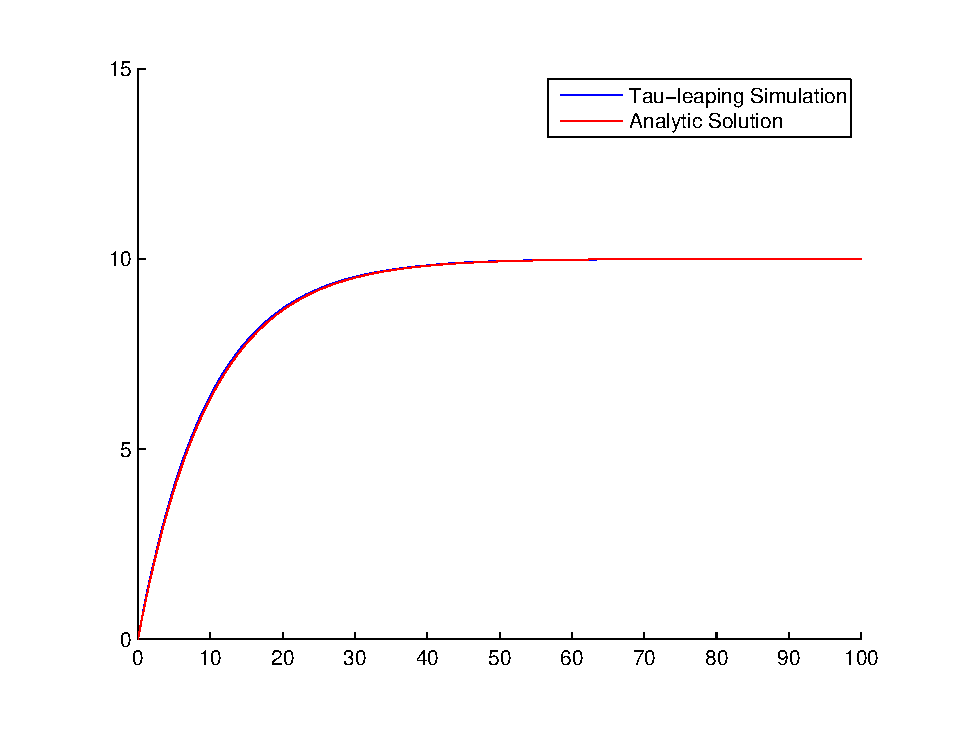
\includegraphics[width=\textwidth]{images/prod_deg_time.eps}
\caption{Analytic solution of the production-degradation system \eqref{eq:gendeg1}-\eqref{eq:gendeg2} and average of $128^3=2097152$ tau-leaping simulations. Parameterization: $k_1 = 0.1$, $k_2 = 1$, $a(0) = 0$, $\epsilon = 0.05$}
\label{fig:prod_deg_time}
\end{figure}

\begin{figure}
\centering
\includegraphics[width=\textwidth]{images/prod_deg_hist.eps}
\caption{Histogram of the production-degradation system \eqref{eq:gendeg1}-\eqref{eq:gendeg2}. Parameterization analogous to figure \ref{fig:prod_deg_time}. }
\label{fig:prod_deg_hist}
\end{figure}

\paragraph{2D heat equation} In order to validate the diffusion mechanism of the stochastic simulators the parabolic partial differential equation know as heat equation (in this context also called diffusion equation) is considered:
\begin{align}
\frac{\partial \rho(x,y,t)}{\partial t} = D \Delta \rho(x,y,t)=D\left(\frac{\partial^2 \rho(x,y,t)}{\partial x^2} + \frac{\partial^2 \rho(x,y,t)}{\partial y^2}\right)
\label{eq:heat}
\end{align}
$\rho(x,y,t)$ can either be considered the amount of heat or the concentration of some species at time $t$ in a point at $(x,y)$. The diffusion constant $D$ is a positive constant. To facilitate visualization two-dimensional diffusion is considered. 

The domain $\Omega$ shall be the unit square, i.e.} $x,y\in[0,1]$. The system is endowed with Dirichlet boundary conditions
\begin{align}
\rho(0,y,t)=\rho(x,0,t)=\rho(1,y,t)=\rho(x,1,t)=0 \;t>0
\label{eq:heatboundary}
\end{align}
and an initial distribution
\begin{align}
\rho(x,y,0) = \sin(x\pi) \cdot \sin(y\pi)
\label{eq:heatinit}
\end{align}

Under these conditions an analytic solution can be obtained:
\begin{align}
\rho(x,y,t) = \sin(x\pi= \cdot \sin(y\pi) \cdot \exp(-2\pi^2Dt)
\end{align}

Figures \ref{fig:diff_analytic} and \ref{fig:diff_stoch} show the state of the system ($D=10^{-3}$) at $t=60$ obtained by the analytic solution and tau-leaping stochastic simulation, respectively. For the latter 128x128 compartments, the accuracy control parameter $\epsilon = 0.05$ and the scaling constant $\Omega = 1000$ were used. 

The number of molecules is proportional to the volume integral over concentration. For the 2D case one has the following area integral: 
\begin{align}
C_{analytic} = \int_0^1 \int_0^1 \rho(x,y,60) = \frac{4}{\pi^2}\cdot \exp(-0.12\cdot \pi^2) \approx 0.12399
\end{align}
For the democratized stochastic approach it is equivalent to consider the sum over all compartments:
\begin{align}
C_{discrete} = \cdot \sum_{i,j} v_{i,j} \cdot \frac{x_{i,j}}{\Omega}
\end{align}
where $v$ is the volume of the compartment and $x$ the number of molecules in it. Considering the presented two-dimensional example with 128x128 uniform square-shaped compartments one has for the absolute error $\Delta C = \abs{C_{analytical} - C_{discrete}} \approx 1.4232\cdot10^{-5}$, for the relative error $\delta C = \Delta C / C_{analytic} \approx 1.1478\cdot 10^{-4}$.  

\begin{figure}
\centering
% l b r t
\includegraphics[trim = 15mm 0mm 10mm 35mm, clip, width=3cm,width=\textwidth]{images/diff_analytic.png}
\caption{Analytic solution of heat equation \eqref{eq:heat} for $D=10^{-3}$ with boundary condition \eqref{eq:heatboundary} and initial condition \eqref{eq:heatinit} at $t=60$.}
\label{fig:diff_analytic}
\end{figure}

\begin{figure}
\centering
% l b r t
\includegraphics[trim = 15mm 0mm 10mm 35mm, clip, width=3cm,width=\textwidth]{images/diff_stoch.png}
\caption{Stochastic solution of heat equation \eqref{eq:heat} for $D=10^{-3}$ with boundary condition \eqref{eq:heatboundary} and initial condition \eqref{eq:heatinit} at $t=60$. Parameterization: $\epsilon = 0.05$, $\Omega = 1000$, spacing h=1/127}
\label{fig:diff_stoch}
\end{figure}


%\section{Pattern formation in the Gray-Scott System}
\section{Pattern formation in the Gray-Scott System}
One of the main reasons for the great interest in the Gray-Scott model is its ability to develop complex spatio-temporal patterns. Pattern formation is a form of self-organization which plays a central role in a variety of processes observed in nature that are crucial for the existence of live in any form (see chapter \ref{ch:intro} for examples). In this section it is shown how the developed stochastic simulator can be used to illustrate the temporal evolution of the system. 

The following initial conditions for the number of particles of species U and V are used throughout the whole thesis:
\begin{align}
 u_0 =
  \begin{cases} 
      \hfill    \Omega \left( \frac{1}{2} + \xi\cdot 10^{-2} \right) \hfill & \text{ if $\mathcal{G}_{int}$} \\
      \hfill \Omega \left( 1 + \xi \cdot 10^{-2} \right) \hfill & \text{ otherwise} \\
  \end{cases}
\end{align}
and
\begin{align}
 v_0 =
  \begin{cases} 
      \hfill    \Omega \left( \frac{1}{4} + \xi\cdot 10^{-2} \right) \hfill & \text{ if $\mathcal{G}_{int}$} \\
      \hfill \Omega \left( \xi \cdot 10^{-2} \right) \hfill & \text{ otherwise} \\
  \end{cases}
\end{align}
with random variable $\xi\! \sim\! \operatorname{Unif}(0,1)$ and inner region $\mathcal{G}_{int} = [1/4, 3/4]^d$ where $d$ is the dimension of the system under consideration. The initial conditions were chosen in dependence on \ref{rossinelli_accelerated_2008}. The parameters used are $F=0.04$, $\kappa = 0.06$, $\rho_d = 1-0$ (i.e.\ $\rho_s = 2.0$), $D_u = 2\cdot 10^{-4}$. 

Figure \ref{fig:pattern} illustrates the influence of the scaling parameter $\Omega$. For large values (e.g.\ $\Omega \gtrsim 10000$), the system is close to the thermodynamic limit, i.e.\ the deterministic approach is a valid approximation to the stochastic microscopic phenomena \ref{gillespie_deterministic_2009}. Figure \ref{todo} gives insight into the temporal evolution of the system, figure \ref{fig:3d} shows the isosurface for the concentration of species U at time $t=1000$ with respect to an isovalue of $0.5$. 

\begin{figure}
\centering
\includegraphics[height=0.4\paperheight]{images/3d.png}
\caption{Isosurface representation of the concentration of species U at $t=1000$ for an isovalue of 0.5.}
\label{fig:3d}
\end{figure}

In the literature and on the Internet numerous articles and websites on Gray-Scott pattern formation exist. Two especially illustrative resources on the topic shall be mentioned here: Project \textit{Xmorphia}\footnote{Original website unavailable. Extended version by R. Munafo: \url{http://goo.gl/vFnOU8}} by Roy Williams at Caltech and the \textit{Amorphous Computing}\footnote{\url{http://goo.gl/4iZUb1}} project by Abelson et al.\ at MIT CSAIL. Both websites enable interactive exploration of the system behaviour under different conditions. The former resource includes a map of the parameter space which directly links to videos that visualize the temporal evolution of the system for the selected setup. The latter includes interactive simulators and videos that illustrate the great variety of patterns that can be obtained. 

%Figure temporal evolution like previous

\begin{figure}
\centering
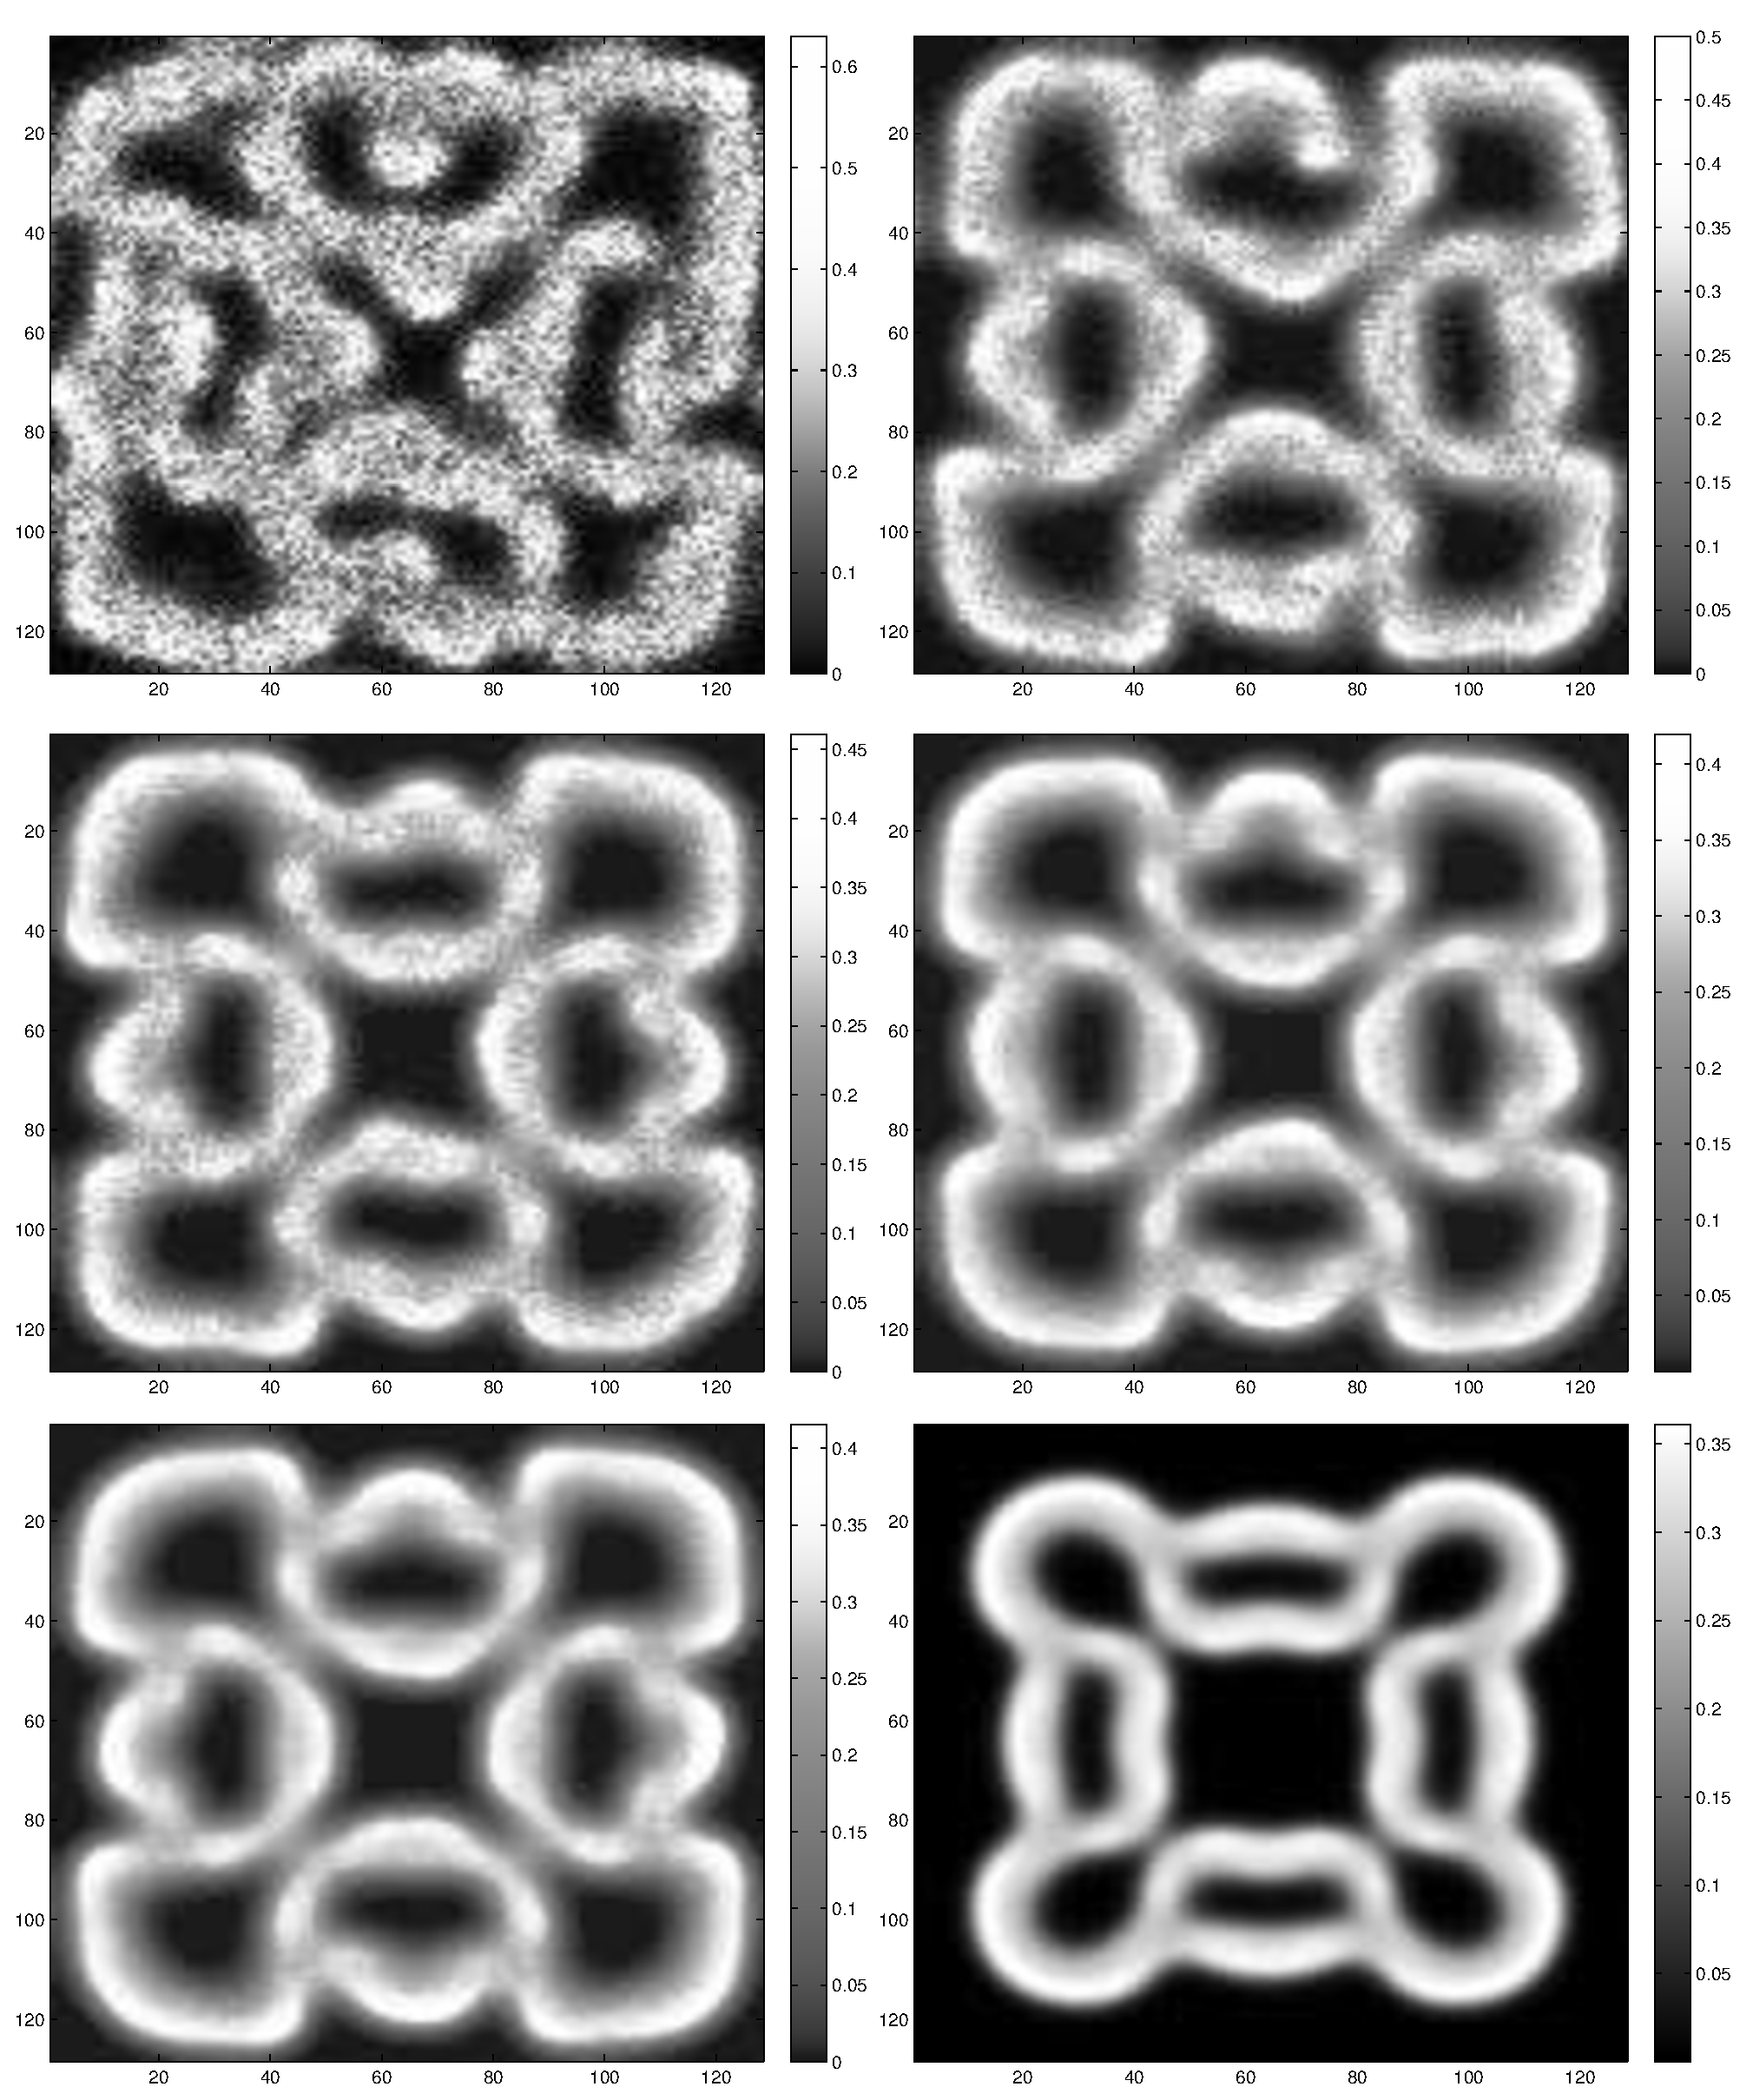
\includegraphics[width=\textwidth]{images/pattern.eps}
\caption{Pattern formation under the influence of varying molecule numbers. Figure shows simulation domain $[0,1]^3$ at time $t=1000$ divided in $128^3$ compartments and sliced at $x=0.6$. Parameters $F=0.04$, $\kappa = 0.06$, $\rho_d = 1-0$ (i.e.\ $\rho_s = 2.0$), $D_u = 2\cdot 10^{-4}$ and $D_v = 1\cdot 10^{-5}$ are used. From left to right and top to bottom the following values for $\Omega$ are used: 100, 500, 1000, 5000, 10000. The plot in the bottom right corner shows the deterministic solution (subject to finite-amplitude random perturbation) obtained with a finite difference approximation. Accuracy control parameter: $\epsilon = 0.05$}
\label{fig:pattern}
\end{figure}
%\section{Performance Analysis}
\section{Performance Analysis}
\label{ch:perf}
Simulation platforms: GTX 580, ...
% a9xxx : 3rd-generation nodes (2011) with 4 12-core AMD Opteron 6174 CPUs and InfiniBand network

\paragraph{Optimization of the GPU version} \label{ch:gpuopt} A GPU is a powerful but highly complex device. In order to ensure that an application uses the available resources efficiently performance evaluation and iterative optimization must be an integral part of the development process. The CUDA framework comes with advanced profiling tools (e.g.\ the Nvidia Visual Profiler) that automatically detect some of the worst pitfalls in GPU programming and can support the developer in trying to avoid them. 


In the following some optimization ideas that arouse during the development process of the GPU tau-leaping simulator are discussed. 

\begin{description}
\item[Initial] In chapter \ref{ch:gpuimplementation} three different approaches towards implementing diffusion were presented. In table \ref{tab:opti} execution times of one complete simulation step (i.e.\ tau calculation, reaction and diffusion) are given for each of the variants. As expected, the naive kernel performs worst since it does not used fast shared memory. The fact that \texttt{kernel\_shared} outperforms the more sophisticated alternative \texttt{kernel\_four}, on the other hand, might be surprising. In \ref{atomics} it has been shown that atomic operations on CUDA-enabled GPUs are significantly slower than regular memory transactions (up to 100x). In reality, however, it seems that the slowdown due to the overhead of three additional kernel launches and a more irregular access pattern overweights the benefits of avoiding atomics in global memory. The main reason for this result is definitely the accelerated hardware support for atomic operations in modern GPUs such as the Nvidia GeForce GTX 580 (in general compute capability $\geq$ 2.0). Another contributing factor is the small degree of the worst case collision, i.e.\ a maximum of four threads can possibly access a value in global memory at the same time. On GPUs it is often the case that a simple, computationally more expensive algorithm with simple control flow outperforms a complex, more efficient implementation that would be faster on a CPU. In the following only \texttt{kernel\_shared} is considered since it performed best in all stages of development and in the final simulator. 
\item[Combination of reaction and diffusion] As mentioned before the reaction and the diffusion operation can be merged. All information that is needed for simulating the local reactions is available within the diffusion kernel. Consequently the overhead of one kernel launch and more importantly several costly operations in global memory can be avoided. The relative speedup of this optimization is $\approx 4.3\%$. 
\item[Register count optimization] In chapter \ref{ch:gpuimplementation} the remark has been made that multiprocessor registers have to be considered a valuable resource in GPGPU computing. The reason will become obvious now: The original implementation of the reaction-diffusion kernel occupies 63 registers. Considering a block size of 512 threads (i.e.\ a 8x8x8 grid is used to reduce the number of global memory atomic operations) and 32768 registers that are available on each SM, only one block can reside on it at a time. This means that the number of threads that are available for execution in case a warp stalls to wait for a memory transaction is limited. As a result of the low \textit{occupancy} memory latency cannot be hidden by fast context switching. By using switches such as \texttt{-maxrregcount} the compiler can be forced to reduce the number of registers occupied by the kernel. Values that do not fit into registers any more are spilled to global memory. Trying to hide global memory latency by spilling variables to global memory may sound strange, but since heavily used values are kept in a on-chip L1 cache the approach is promising. By limiting the number of registers per thread to 31 two blocks can be scheduled per SM at the same time. The relative speedup obtained for the tau-leaping simulator is 11.2\%. 

It it obvious that the best alternative to forcing the compiler to lower register counts is not using a great number of registers in the first place. In a complex kernel such as the three-dimensional reaction-diffusion example where local as well as global boundary conditions and special cases have to be handled and comparably large PRNG states have to be kept in local memory reducing the number of registers is a nontrivial task. In future work together with improved compilers that apply more advanced optimization techniques based on compile time knowledge and control flow analysis a further increase in performance can be obtained. 

\item[Increase work per thread] Even in a framework such as CUDA that heavily relies on data parallelism a solution that exposes as much concurrent work as possible might not be the fastest. A good example for this optimization approach can be found in an example by Nvidia's Mark Harris \cite{nvidia reduction}. For the reaction-diffusion kernel under consideration it turns out that the average execution time of a simulation steps is minimized if every thread handles 16 compartments. This values has been obtained by heuristic experiments and depends on GPU generation and model. For the concrete example a considerable relative speedup of 39\% is achieved. 
\end{description}

\begin{table}[]
\centering
\newcolumntype{d}[1]{D{.}{\cdot}{#1} }
\begin{tabular}{|l|r|r|}
\hline
 \textbf{Optimization} & \textbf{Time / simulation step (ms)} & \textbf{Relative speedup}\\ \hline
 Initial (naive) & 21.98 & --- \mbox{     }\\ \hline
 Initial (shared) & 16.78 & --- \mbox{     }\\ \hline
 Initial (four) & 18.35 & --- \mbox{     }\\\hline
 Combination R\&D & 16.06 & 4.3\% \\ \hline
 Register count & 14.26 & 11.2\% \\ \hline
 Work per thread &  8.70 & 39.0\% \\ \hline
\end{tabular}
\caption{Execution time per simulation step and relative speedup of selected optimization steps. Absolute times are negatively affected by the performance measurement itself since additional synchronization is needed. Values obtained during the standard 128x128x128 compartment simulation of the Gray-Scott model. }
\label{tab:opti}
\end{table}

\paragraph{Optimization of the CPU version} Due to the rather coarse grained task parallelism approach of OpenMP optimizing methods for the CPU version are limited. Avoiding the overhead of one fork-join operation per step by introducing one large parallel region reduces the execution time per step by approximately 50\% (1.05s vs.\ 0.54s on an Intel Core i5-2430M with four threads\ref{todo check consistency}). Further optimization techniques may involve the use of vector instructions (SSE, AVX) or the introduction of cache-optimized access patterns (tiling, space-filling curve). Those techniques are highly complex to implement and far beyond scope. In this thesis the potential of two parallel platforms for accelerating stochastic simulations in time-limited academic projects is assessed. In this framework an optimal solution in terms of efficiency is neither possible to achieve nor a necessity. 

\paragraph{GPU strong domainsize} Medium sized system: performance leader \\
by no means perfect: peak throughput: schoenrechnen \\

\paragraph{CPU scaling number of threads} Memory limited and scaling

\paragraph{resume} Difference factor. But in reality highly optimized version. CUDA forces developer to vectorize, makes it easy. 

\ifdebug
1. 1 second simulation of tau leaping cpu 1-48 threads and naive, chessboard
2. GPU optimization steps
3. gpu scaling: size of system
3. same system



\begin{itemize}
\item Cite 'Debunking ...'
\item Speedup GPU vs.\ CPU
\item Bandwith vs. theoretical
\item Ideas to optimize
\end{itemize}
Simulation Performance?
\begin{itemize}
\item deviceQuery GTX 580 (global memory: 1535 MB, 16 SM, 32 CC/SM, GPU clock 1,62 GHz, Memory CR 2016 MHz, M Bus Width 384-bit, Smem / block: 49152 bytes, registers per block 32768, tpb 1024, tpSM 1536)
\item Time per step
\item Time to solution
\item Bandwidth estimation
\item FLOP/s from cuvpp?
\item Optimizations: Approaches to diffusion
\item Occupancy: PTX, ...
\item Several cells per block
\item GPU outperforms CPU by a factor of 25x to 100x (Nobile)
\end{itemize}

\ifdebug
Optimization: Reduce # register -> occupancy -> hide latency
\fi

\ifdebug
\section{Comparison of of both systems and implications on implementation strategies}
fields of application

\begin{itemize}
\item No complex memory hierarchy
\item Tiling is natural on GPU
\item ...
\item data level parallelism vs.\ thread parallelism
\end{itemize}
rule of thumb: complex control flow: cpu, simple control view, parallelizable, vectorization, data centric
\fi
\fi
\chapter{Conclusion and Outlook}
\label{ch:outlook}
\chapterprecishere{"I think and think for months and years. Ninety-nine times, the conclusion is false. The hundredth time I am right."}{\hfill -- Albert Einstein \cite{betterlife}}

What has been done. \\
Both implementations are not perfect. GPUs are reasonable to use. Worth it to learn. Important skill. Learning ot think in parallel is necessary. \\
Results: GPU beets CPU for medium sized problems. Interesting devices. Trend: dynamic parallelism\\
But don't underestimate the potential of CPUS. Future: Xeon Phi \\
Stochastic algorithms are great, examples from several scales (universe, cell, ...). \\
Tau-leaping outperforms classic approaches that consider every individual particle. (more comple implementation) \\
Computational methods are valuable tool, enables understanding dynamic evolution of biological systems, global-level understanding of emergent dynamics... \\
\chapter{Acknowledgment}
First of all sincere gratitude goes to my supervisor Jana Lipkov\'a. The contribution of her friendly support and helpful suggestions to this thesis cannot be overestimated. 
Furthermore, I would like to express my very great appreciation to Petros Koumoutsakos for giving me the opportunity to write this Bachelor's thesis in his lab. 

I would like to offer my special thanks to my mentors Hans-Joachim Bungartz and Klaus Mainzer at TUM. Their support before and during my semester in Zurich was enormously beneficial. Professor Mainzer's guidance concerning potential topics for this thesis is greatly appreciated. My thanks to Professor Bungartz for being supervisor to this thesis, for his support with administrative matters in Munich and Zurich as well as for his valuable advice on future studies cannot be overemphasized. 

Last but by no means least assistance provided by Gerardo Tauriello, Babak Hejazialhosseini and Christiane Pousa Ribeiro is greatly appreciated. 

The semester at ETH was supported by the European Union's Erasmus Program and by the Max Weber-Programme of the sate of Bavaria. 

This thesis is dedicated to my parents, my sister and my girlfriend.

\appendix
\chapter{Steady State Analysis of the Gray-Scott Reaction System}
\label{ch:app1}
\paragraph{Calculation of the steady states}
The steady state condition prescribes 
\begin{align}
\label{app:1}
0 \overset{!}{=} \frac{du}{dt} &= -\rho u v^2 + F(1-u) = f_1(u,v)\\
\label{app:2}
0 \overset{!}{=} \frac{dv}{dt} &= \rho u v^2 - (F + \kappa) v = f_2(u,v)
\end{align}
Combining \eqref{app:1} and \eqref{app:2} leads to
\begin{align}
\label{app:3}
u = 1 - \frac{F + \kappa}{F}
\end{align}
Plugging \eqref{app:3} into \eqref{app:2} gives
\begin{align}
- \frac{F + \kappa}{F} v(v^2 + \rho v - (F + \kappa)) = 0
\end{align}
The trivial steady state is
\begin{align}
\vec{x}_{s1} = 
\begin{bmatrix}
1.0 & 0.0
\end{bmatrix}^T
\end{align}
The two other steady states are
\begin{align}
\vec{x}_{s2/3} = 
\begin{bmatrix}
\frac{1}{2} (1 \pm \sqrt{1 - 4 \frac{(F+\kappa)^2}{F \rho}}) &
\frac{F}{2 (F + \kappa)} (1 \mp \sqrt{1 - 4 \frac{(F + \kappa)^2}{F \rho}})
\end{bmatrix}
\end{align}
For the given parameters ($F = 0.04$, $\kappa = 0.06$ and $\rho = 1.0$) one has
\begin{align}
\vec{x}_{s2} = \vec{x}_{s3} = 
\begin{bmatrix}
0.5 & 0.2
\end{bmatrix}^T
\end{align}

\paragraph{Classification of Eigenvalues}
The Jacobian of the system is
\begin{align}
J = \begin{bmatrix}
\frac{\partial f_1}{\partial u} & \frac{\partial f_1}{\partial v} \\[0.3em]
\frac{\partial f_2}{\partial u} & \frac{\partial f_2}{\partial v}
\end{bmatrix}
=
\begin{bmatrix}
-\rho v^2 - F & -2 \rho u v \\[0.3em]
\rho v^2 & 2 \rho u v - (F + \kappa)
\end{bmatrix}
\end{align}
For the given parameters and at the steady state $\vec{x}_{s1}$ this is
\begin{align}
J_{s1} = \begin{bmatrix}
-0.04 & 0 \\
0 & -0.1
\end{bmatrix}
\end{align}
The eigenvalues of this matrix are $\lambda_{11} = -0.1$ and $\lambda_{12} = -0.04$. Since $\Re(\lambda_{11}) < 0$ and $\Re(\lambda_{12}) < 0$ this steady state is stable. \par
For the given parameters and the steady states $\vec{x}_{s2} = \vec{x}_{s3}$ this is
\begin{align}
J_{s2} = J_{s3} = 
\begin{bmatrix}
-0.08 & -0.2 \\
0.04 & 0.1
\end{bmatrix}
\end{align}
The eigenvalues of this matrix are the roots of the characteristic polynomial
\begin{align}
(-0.08-\lambda)(0.1-\lambda)+0.08=\lambda (\lambda - 0.02)
\end{align}
One obtains $\lambda_{21} = \lambda_{31} = 0$ and $\lambda_{22} = \lambda_{32} = 0.02$.
%
%
%
%
%

\backmatter

\bibliographystyle{alpha}
%plain, alpha, apalike
\bibliography{refs}

% \includepdf[pages=-]{do.pdf}

\end{document}